\chapter{Verification and Evaluation of the \textit{i}MGXS Scheme}
\label{chap:results}

first paragraph: objective
-recall two primary objectives:
  -approach null convergence rate
  -achieve degenerate's accuracy

-recall Chaps 8 and 9 results:
  -all schemes produce the same eigenvalue
  -clustering MGXS largely inconsequential for pin-wise fission rates
  -clustering MGXS very important for accurate U-238 capture rates
  -deterministic LNS scheme worked well, but suffers from two main flaws:
    -not flexible for arbitrary geometries (e.g., reflectors, baffles)
    -not scalable for large geometries

-recall Chap. 10:
  -developed \textit{i}\ac{MGXS} to circumvent the above issues with LNS

-TWO PRONGED OBJECTIVE HERE:
  1) Verify iMGXS scheme - make sure everything works as expected
  2) Quantify accuracy wrt degenerate case
  3) Quantify convergence rate of OpenMOC results with \textit{i}\ac{MGXS} 
  4) Evaluate model selection criteria


\begin{figure}[h!]
\centering
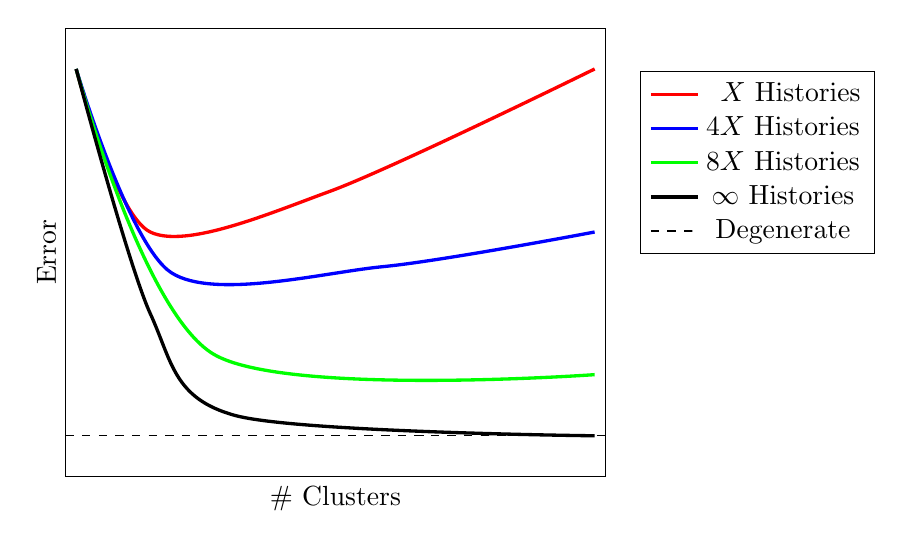
\begin{tikzpicture}
\begin{axis}[xmin=0,xmax=51,ymin=0,ymax=1.1,xlabel={\# Clusters},ylabel={Error},xticklabels={},yticklabels={},xtick={},ytick={},ticks=none,legend style={at={(1.5,0.7)},anchor=east,legend columns=1}]
\addplot[smooth,red,very thick] coordinates {
(1,1)
(8,0.6)
(25,0.7)
(50,1)
};
\addplot[smooth,blue,very thick] coordinates {
(1,1)
(10,0.5)
(30,0.515)
(50,0.6)
};
\addplot[smooth,green,very thick] coordinates {
(1,1)
(14,0.3)
%(30,0.45)
(50,0.25)
};
\addplot[smooth,very thick] coordinates {
(1,1)
(8,0.4)
(16,0.15)
(50,0.1)
};
\addplot[smooth,dashed] coordinates {
(0,0.1)
(51,0.1)
};
\addlegendentry{$\;\;X$ Histories}
\addlegendentry{$4X$ Histories}
\addlegendentry{$8X$ Histories}
\addlegendentry{$\infty$ Histories}
\addlegendentry{Degenerate}
\end{axis}
\end{tikzpicture}
\caption[Convergence of\textit{i}MGXS to degenerate homogenization]{Convergence of \textit{i}\ac{MGXS} to degenerate homogenization in the limit of infinite particle histories.}
\label{fig:chap11-coverge-complexity}
\end{figure}

%%%%%%%%%%%%%%%%%%%%%%%%%%%%%%%%%%%%%%%%%%%%%%%%%%%%%%%%%%%%%%%%%%%%%%%%%%%%%%%
\section{MOC Runtime Parameters}
\label{sec:chap11-moc-params}

-need to discuss parameters for batchwise 
-only 70 groups per the results from preceding chapters
-128 angles, 0.05 cm track spacing as always
-10$^{-5}$ convergence tolerance on the \ac{FSR} fission source as always
-FSR discretization for each benchmark same as detailed in Sec.~\ref{subsec:chap8-fsr-discretizations}

%%%%%%%%%%%%%%%%%%%%%%%%%%%%%%%%%%%%%%%%%
\section{Analysis of Multi-Group Results}
\label{subsec:chap11-imgxs-bias}

first paragraph: OpenMC MGXS generation:
-100,000 particles / batch - individual assemblies
-400,000 particles / batch - 2x2 and reflector??
-1,000,000 particles / batch - quarter core
-10,000 batches for assemblies and reflector
-how many batches for full core??
-results may differ somewhat from those for null, degenerate and LNS schemes:
  -also used 1E9 total histories to evaluate other homogenization schemes
  -but those used 1E6 particles / batch, and thus only 8E8 active histories
  -these results are for 9.9E8 active histories since fewer particles per inactive batch

second paragraph: outline
-don't report on fission rates here
-Sec.~\ref{subsec:chap11-imgxs-eigenvalue-bias}
-Sec.~\ref{subsec:chap11-imgxs-capt-rates}

%%%%%%%%%%%%%%%%%%%%%%%%%%%%
\subsection{Eigenvalue Bias}
\label{subsec:chap11-imgxs-eigenvalue-bias}

first paragraph: outline
-methodology:
  -recall pinch and litmus-only feature selection
  -recall four clustering algorithms
-eigenvalues should match those for null, degenerate and LNS schemes
  -don't expect clustering algorithm to have any impact on the eigenvaue bias

second paragraph: outline and analysis
-Tab.~\ref{table:chap11-eigenvalues-litmus-only}
  -benchmark
  -clustering algorithm
  -number of clusters
-remark on consistency for eigenvalues irregardless of number of clusters and clustering algorithm

-perhaps reduce number of columns in table to null, degenerate, LNS, and 2, and 6 clusters??
  -determine clusterings to columnize from plots of U-238 capture rate errors by \# clusters

\begin{table}[ht!]
  \centering
  \caption[OpenMOC eigenvalue bias for litmus-only feature selection]{OpenMOC eigenvalue bias $\Delta\rho$ for \textit{i}\ac{MGXS} spatial homogenization with litmus-only feature selection.}
  \small
  \label{table:chap11-eigenvalues-litmus-only}
  \vspace{6pt}
  \begin{tabular}{l l R{1.5cm} R{1.5cm} R{1.5cm} R{1.5cm} R{1.5cm}}
  \toprule
  \rowcolor{lightgray}
  & \multicolumn{1}{c}{\cellcolor{lightgray} \bf Clustering} & \multicolumn{5}{S[table-format=6.1]}{\cellcolor{lightgray} \textbf{\# Clusters}} \\
  \multirow{-2}{*}{\cellcolor{lightgray} \bf Benchmark} &
  \multicolumn{1}{c}{\cellcolor{lightgray} \bf Algorithm} &
  \multicolumn{1}{c}{\cellcolor{lightgray} \bf 2} &
  \multicolumn{1}{c}{\cellcolor{lightgray} \bf 4} &
  \multicolumn{1}{c}{\cellcolor{lightgray} \bf 6} &
  \multicolumn{1}{c}{\cellcolor{lightgray} \bf 8} &
  \multicolumn{1}{c}{\cellcolor{lightgray} \bf 10} \\
  \midrule
\multirow{4}{*}{\parbox{2.5cm}{1.6\% Assm}} & Agglomerative & -168 & -168 & -168 & -168 & -168 \\
& BIRCH & -168 & -168 & -168 & -168 & -168 \\
& \ac{GMM} & -168 & -168 & -168 & -168 & -168 \\
& $k$-means & -168 & -168 & -168 & -168 & -168 \\
  \midrule
\multirow{4}{*}{\parbox{2.5cm}{3.1\% Assm}} & Agglomerative & -194 & -194 & -194 & -194 & -194 \\
& BIRCH & -194 & -194 & -194 & -194 & -194 \\
& \ac{GMM} & -194 & -194 & -194 & -194 & -194 \\
& $k$-means & -194 & -194 & -194 & -194 & -194 \\
  \midrule
\multirow{4}{*}{\parbox{2.5cm}{3.1\% Assm w/ 20 \acp{BP}}} & Agglomerative & -237 & -236 & -235 & -235 & -235 \\
& BIRCH & -237 & -236 & -235 & -235 & -235 \\
& \ac{GMM} & -236 & -235 & -236 & -235 & -235 \\
& $k$-means & -236 & -236 & -236 & -235 & -235 \\
  \midrule
\multirow{4}{*}{\parbox{2.5cm}{2$\times$2 Colorset}} & Agglomerative & -189 & -189 & -189 & -189 & -189 \\
& BIRCH & -189 & -189 & -189 & -189 & -189 \\
& \ac{GMM} & -188 & -189 & -188 & -189 & -189 \\
& $k$-means & -188 & -189 & -188 & -189 & -189 \\
  \midrule
\multirow{4}{*}{\parbox{2.5cm}{2$\times$2 Colorset w/ Reflector}} & Agglomerative & -136 & -136 & -134 & -129 & -133 \\
& BIRCH & -138 & -137 & -136 & -133 & -133 \\
& \ac{GMM} & -136 & -136 & -137 & -133 & -133 \\
& $k$-means & -136 & -136 & -134 & -132 & -132 \\
  \midrule
\multirow{4}{*}{\parbox{2.5cm}{BEAVRS Quarter Core}} & $k$-Means & & & & & \\
& Agglomerative & & & & & \\
& BIRCH & & & & & \\
& GMM & & & & & \\
  \bottomrule
\end{tabular}
\end{table}

\clearpage

%%%%%%%%%%%%%%%%%%%%%%%%%%%%%%%%
\subsection{U-238 Capture Rates}
\label{subsec:chap11-imgxs-capt-rates}

first paragraph: outline
-methodology:
  -recall pinch and litmus-only feature selection
  -recall four clustering algorithms
-looking for two things:
  -1) want U-238 capture rates as accurate as the degenerate case
    -perhaps even more accurate if MGXS are ``de-noised'', as was observed for LNS??
  -2) want to out-perform LNS for 2$\times$2 color with reflector and quarter core
  -3) want to compare different OpenMOC solutions to see relative impact of clustered \ac{MGXS}

second paragraph: outline

third paragraph: analysis
-differences between number of clusters
-differences between clustering algorithms
-differences between litmus-only and pinch feature selection

-should mention errors with ICA, PCA, or FA to illustrate that clustering can screw up??? 

%%%%%%%%%%%%%%%%%%%%%%%%%%%%%%%%%%%%%%%%%%%%%%%%%%%%%
\subsubsection{Variation with the Number of Clusters}
\label{subsec:chap11-imgxs-capt-rates-num-clusters}

-figures of capture rate percent relative errors by number of clusters
  -benchmark
  -clustering algorithm
  -number of clusters

\begin{figure}[h!]
\centering
\begin{subfigure}{0.9\textwidth}
  \centering
  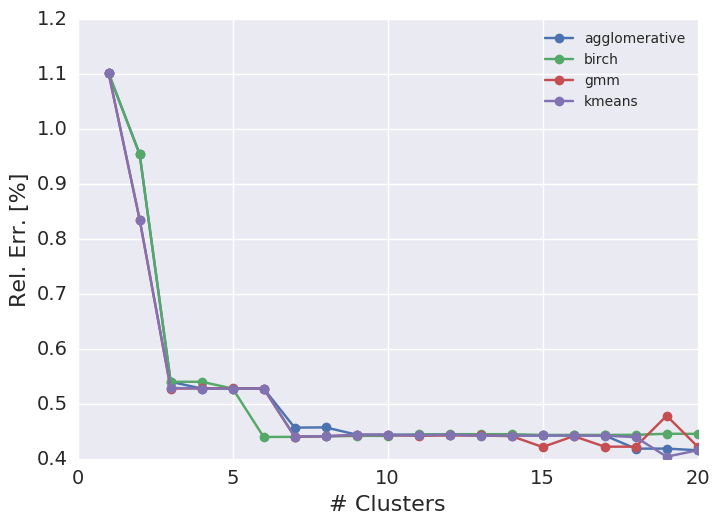
\includegraphics[width=\linewidth]{figures/results/err-by-cluster/assm-16/max-rel-err}
  \caption{}
  \label{fig:chap11-max-capt-err-by-cluster-assm-16}
\end{subfigure}
\begin{subfigure}{0.9\textwidth}
  \centering
  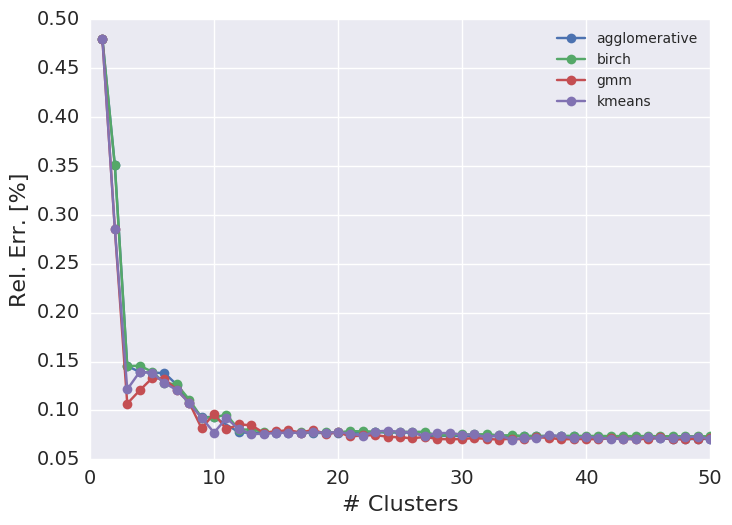
\includegraphics[width=\linewidth]{figures/results/err-by-cluster/assm-16/mean-rel-err}
  \caption{}
  \label{fig:chap11-mean-capt-err-by-cluster-assm-16}
\end{subfigure}
\caption[U-238 capture rate errors for the 1.6\% enriched assembly]{The max (a) and mean (b) U-238 capture rate errors for the 1.6\% enriched assembly with \textit{i}\ac{MGXS} spatial homogenization with litmus-only feature selection.}
\label{fig:chap11-capt-err-by-cluster-assm-16}
\end{figure}

\begin{figure}[h!]
\centering
\begin{subfigure}{0.9\textwidth}
  \centering
  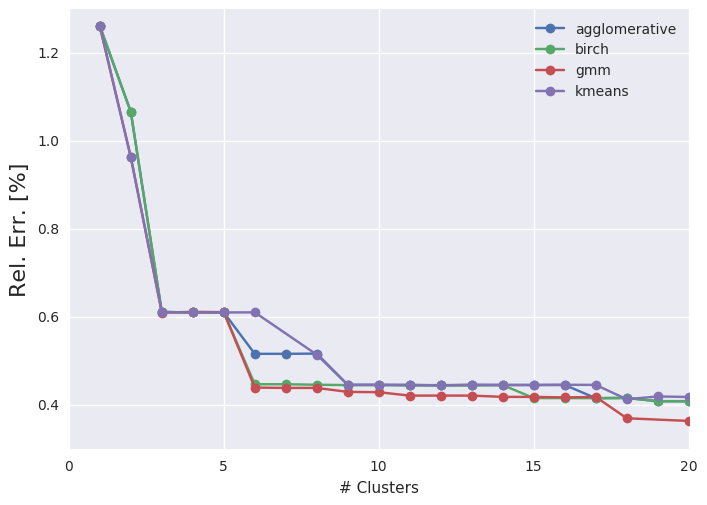
\includegraphics[width=\linewidth]{figures/results/err-by-cluster/assm-31/max-rel-err}
  \caption{}
  \label{fig:chap11-max-capt-err-by-cluster-assm-31}
\end{subfigure}
\begin{subfigure}{0.9\textwidth}
  \centering
  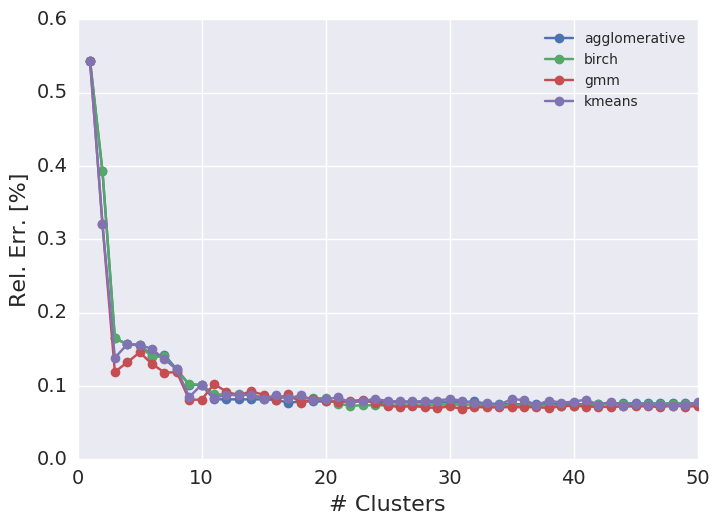
\includegraphics[width=\linewidth]{figures/results/err-by-cluster/assm-31/mean-rel-err}
  \caption{}
  \label{fig:chap11-mean-capt-err-by-cluster-assm-31}
\end{subfigure}
\caption[U-238 capture rate errors for the 3.1\% enriched assembly]{The max (a) and mean (b) U-238 capture rate errors for the 3.1\% enriched assembly with \textit{i}\ac{MGXS} spatial homogenization with litmus-only feature selection.}
\label{fig:chap11-capt-err-by-cluster-assm-31}
\end{figure}

\begin{figure}[h!]
\centering
\begin{subfigure}{0.9\textwidth}
  \centering
  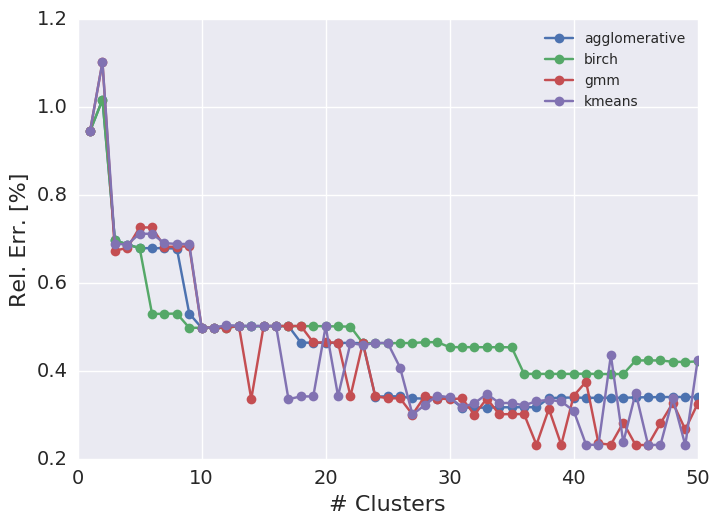
\includegraphics[width=\linewidth]{figures/results/err-by-cluster/assm-31-20BPs/max-rel-err}
  \caption{}
  \label{fig:chap11-max-capt-err-by-cluster-assm-31-20BPs}
\end{subfigure}
\begin{subfigure}{0.9\textwidth}
  \centering
  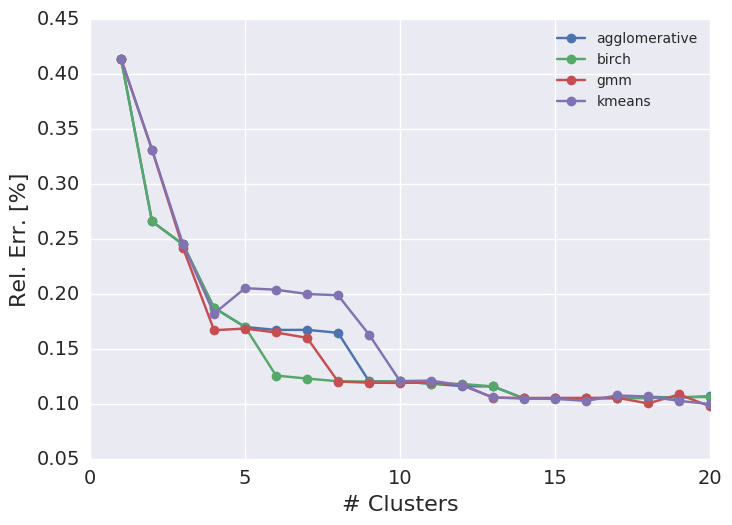
\includegraphics[width=\linewidth]{figures/results/err-by-cluster/assm-31-20BPs/mean-rel-err}
  \caption{}
  \label{fig:chap11-mean-capt-err-by-cluster-assm-31-20BPs}
\end{subfigure}
\caption[U-238 capture rate errors for the 3.1\% enriched assembly with 20 BPs]{The max (a) and mean (b) U-238 capture rate errors for the 3.1\% enriched assembly with 20 \acp{BP} with \textit{i}\ac{MGXS} spatial homogenization with litmus-only feature selection.}
\label{fig:chap11-capt-err-by-cluster-assm-31-20BPs}
\end{figure}

\begin{figure}[h!]
\centering
\begin{subfigure}{0.9\textwidth}
  \centering
  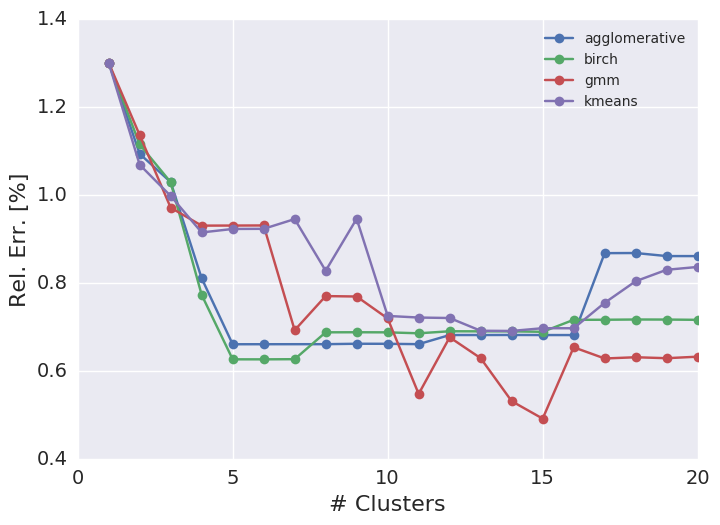
\includegraphics[width=\linewidth]{figures/results/err-by-cluster/2x2/max-rel-err}
  \caption{}
  \label{fig:chap11-max-capt-err-by-cluster-assm-2x2}
\end{subfigure}
\begin{subfigure}{0.9\textwidth}
  \centering
  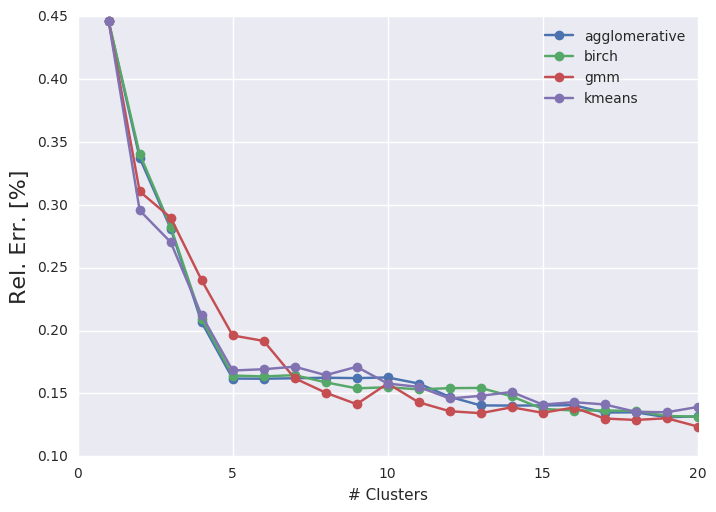
\includegraphics[width=\linewidth]{figures/results/err-by-cluster/2x2/mean-rel-err}
  \caption{}
  \label{fig:chap11-mean-capt-err-by-cluster-assm-2x2}
\end{subfigure}
\caption[U-238 capture rate errors for the 2$\times$2 colorset]{The max (a) and mean (b) U-238 capture rate error for the 2$\times$2 colorset with \textit{i}\ac{MGXS} spatial homogenization with litmus-only feature selection.}
\label{fig:chap11-capt-err-by-cluster-assm-2x2}
\end{figure}

\begin{figure}[h!]
\centering
\begin{subfigure}{0.9\textwidth}
  \centering
  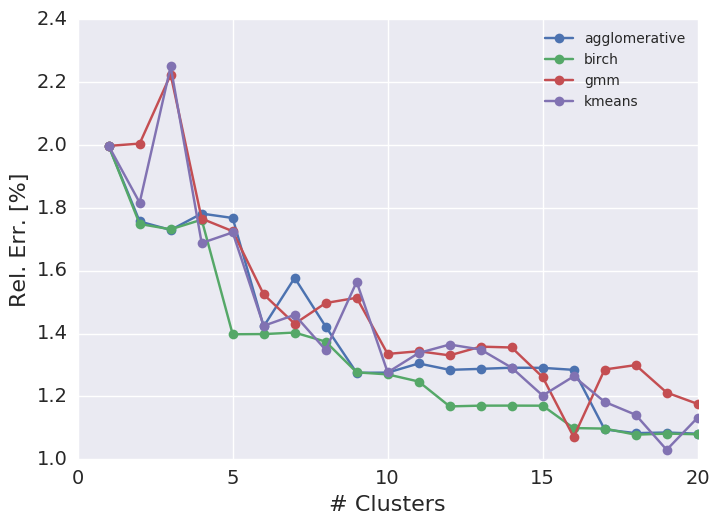
\includegraphics[width=\linewidth]{figures/results/err-by-cluster/reflector/max-rel-err}
  \caption{}
  \label{fig:chap11-max-capt-err-by-cluster-assm-refl}
\end{subfigure}
\begin{subfigure}{0.9\textwidth}
  \centering
  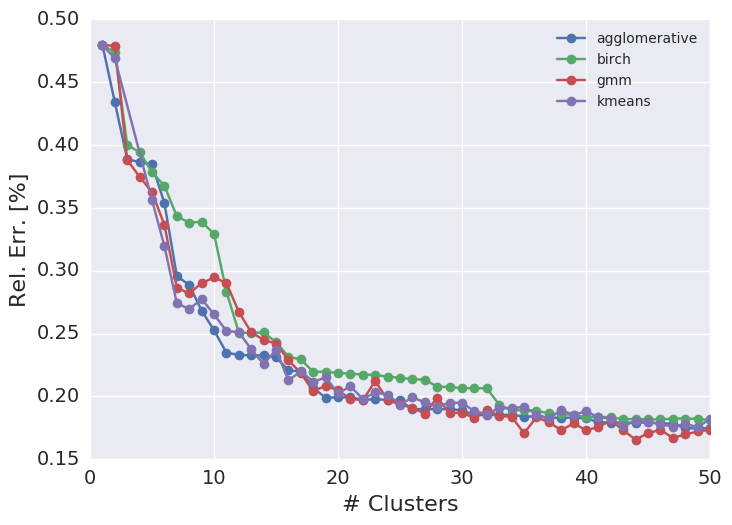
\includegraphics[width=\linewidth]{figures/results/err-by-cluster/reflector/mean-rel-err}
  \caption{}
  \label{fig:chap11-mean-capt-err-by-cluster-assm-refl}
\end{subfigure}
\caption[U-238 capture rate errors for the 2$\times$2 colorset with reflector]{The max (a) and mean (b) U-238 capture rate error for the 2$\times$2 colorset with water reflector with \textit{i}\ac{MGXS} spatial homogenization with litmus-only feature selection.}
\label{fig:chap11-capt-err-by-cluster-assm-refl}
\end{figure}

\begin{figure}[h!]
\centering
\begin{subfigure}{0.9\textwidth}
  \centering
  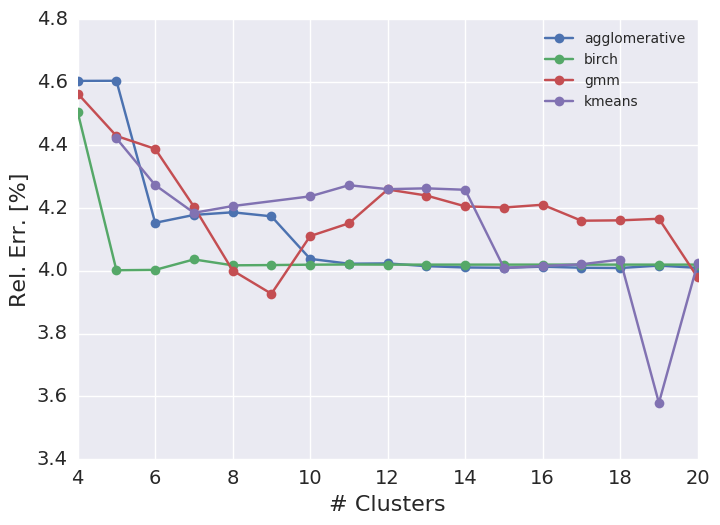
\includegraphics[width=\linewidth]{figures/results/err-by-cluster/full-core/max-rel-err}
  \caption{}
  \label{fig:max-capt-err-by-cluster-assm-full-core}
\end{subfigure}
\begin{subfigure}{0.9\textwidth}
  \centering
  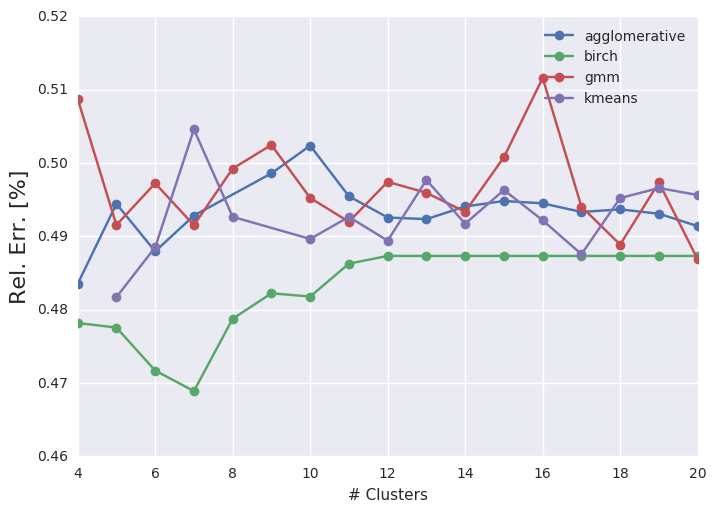
\includegraphics[width=\linewidth]{figures/results/err-by-cluster/full-core/mean-rel-err}
  \caption{}
  \label{fig:mean-capt-err-by-cluster-assm-full-core}
\end{subfigure}
\caption[U-238 capture rate errors for quarter core BEAVRS model]{The max (a) and mean (b) U-238 capture rate error for the quarter core \ac{BEAVRS} model with \textit{i}\ac{MGXS} spatial homogenization with litmus-only feature selection.}
\label{fig:capt-err-by-cluster-assm-full-core}
\end{figure}

SUMMARY BOX

%%%%%%%%%%%%%%%%%%%%%%%%%%%%%%%%%%%%%%%%%%%%%%%%%%%%%%%%%%%%%%
\subsubsection{Benchmark with Null, Degenerate and LNS Schemes}
\label{subsec:chap11-imgxs-capt-rates-benchmark}

-Tabs.~\ref{table:chap11-max-capt-rates-litmus-only} and~\ref{table:chap11-mean-capt-rates-litmus-only}
  -litmus-only feature selection
    -benchmark
    -clustering algorithm
    -number of clusters

\begin{table}[ht!]
  \centering
  \caption[Maximum OpenMOC U-238 capture rate errors for litmus-only feature selection]{Maximum absolute U-238 capture rate percent relative errors for \textit{i}\ac{MGXS} spatial homogenization with litmus-only feature selection.}
  \small
  \label{table:chap11-max-capt-rates-litmus-only}
  \vspace{6pt}
  \begin{tabular}{l l R{1.5cm} R{1.5cm} R{1.5cm} R{1.5cm} R{1.5cm}}
  \toprule
  \rowcolor{lightgray}
  & & \multicolumn{5}{S[table-format=6.1]}{\cellcolor{lightgray} \textbf{\# Clusters}} \\
  \multirow{-2}{*}{\cellcolor{lightgray} \bf Benchmark} &
  \multirow{-2}{*}{\cellcolor{lightgray} \bf Predictor} &
  \multicolumn{1}{c}{\cellcolor{lightgray} \bf 2} &
  \multicolumn{1}{c}{\cellcolor{lightgray} \bf 4} &
  \multicolumn{1}{c}{\cellcolor{lightgray} \bf 6} &
  \multicolumn{1}{c}{\cellcolor{lightgray} \bf 8} &
  \multicolumn{1}{c}{\cellcolor{lightgray} \bf 10} \\
  \midrule
\multirow{4}{*}{\parbox{2.5cm}{1.6\% Assm}} & Agglomerative & 0.955 & -0.529 & -0.529 & -0.458 & -0.445 \\
& BIRCH & 0.955 & -0.541 & -0.441 & -0.442 & -0.443 \\
& \ac{GMM} & -0.836 & -0.529 & -0.529 & -0.442 & -0.444 \\
& $k$-means & -0.836 & -0.529 & -0.529 & -0.442 & -0.445 \\
  \midrule
\multirow{4}{*}{\parbox{2.5cm}{3.1\% Assm}} & Agglomerative & 1.067 & -0.611 & -0.517 & -0.518 & 0.447 \\
& BIRCH & 1.067 & -0.611 & 0.448 & 0.447 & 0.446 \\
& \ac{GMM} & -0.964 & -0.612 & -0.440 & -0.440 & 0.430 \\
& $k$-means & -0.964 & -0.611 & -0.611 & -0.515 & 0.447 \\
  \midrule
\multirow{4}{*}{\parbox{2.5cm}{3.1\% Assm w/ 20 \acp{BP}}} & Agglomerative & -1.017 & 0.688 & 0.680 & 0.679 & -0.499 \\
& BIRCH & -1.017 & 0.688 & -0.531 & -0.531 & -0.499 \\
& \ac{GMM} & -1.102 & 0.680 & 0.727 & -0.531 & -0.499 \\
& $k$-means & -1.102 & 0.687 & 0.713 & -0.691 & -0.499 \\
  \midrule
\multirow{4}{*}{\parbox{2.5cm}{2$\times$2 Colorset}} & Agglomerative & -1.094 & 0.811 & 0.662 & 0.662 & 0.663 \\
& BIRCH & -1.116 & 0.774 & 0.627 & 0.689 & 0.689 \\
& \ac{GMM} & -1.137 & 0.931 & 0.932 & 0.771 & 0.720 \\
& $k$-means & -1.070 & -0.916 & 0.924 & -0.829 & 0.726 \\
  \midrule
\multirow{4}{*}{\parbox{2.5cm}{2$\times$2 Colorset w/ Reflector}} & Agglomerative & -1.757 & -1.782 & -1.423 & -1.423 & -1.276 \\
& BIRCH & -1.749 & -1.763 & -1.399 & -1.374 & 1.270 \\
& \ac{GMM} & -2.005 & -1.766 & -1.525 & 1.497 & -1.335 \\
& $k$-means & -1.817 & -1.688 & -1.425 & 1.348 & -1.277 \\
  \midrule
\multirow{4}{*}{\parbox{2.5cm}{BEAVRS Quarter Core}} & $k$-Means & & & & & \\
& Agglomerative & & & & & \\
& BIRCH & & & & & \\
& GMM & & & & & \\
  \bottomrule
\end{tabular}
\end{table}

\clearpage

\begin{table}[ht!]
  \centering
  \caption[Mean OpenMOC U-238 capture rate errors for litmus-only feature selection]{Mean absolute U-238 capture rate percent relative errors for \textit{i}\ac{MGXS} with litmus-only feature selection.}
  \small
  \label{table:chap11-mean-capt-rates-litmus-only}
  \vspace{6pt}
  \begin{tabular}{l l R{1.5cm} R{1.5cm} R{1.5cm} R{1.5cm} R{1.5cm}}
  \toprule
  \rowcolor{lightgray}
  & & \multicolumn{5}{S[table-format=6.1]}{\cellcolor{lightgray} \textbf{\# Clusters}} \\
  \multirow{-2}{*}{\cellcolor{lightgray} \bf Benchmark} &
  \multirow{-2}{*}{\cellcolor{lightgray} \bf Predictor} &
  \multicolumn{1}{c}{\cellcolor{lightgray} \bf 2} &
  \multicolumn{1}{c}{\cellcolor{lightgray} \bf 4} &
  \multicolumn{1}{c}{\cellcolor{lightgray} \bf 6} &
  \multicolumn{1}{c}{\cellcolor{lightgray} \bf 8} &
  \multicolumn{1}{c}{\cellcolor{lightgray} \bf 10} \\
  \midrule
\multirow{4}{*}{\parbox{2.5cm}{1.6\% Assm}} & Agglomerative & 0.351 & 0.139 & 0.138 & 0.107 & 0.093 \\
& BIRCH & 0.351 & 0.146 & 0.128 & 0.111 & 0.093 \\
& \ac{GMM} & 0.286 & 0.120 & 0.132 & 0.108 & 0.082 \\
& $k$-means & 0.286 & 0.139 & 0.138 & 0.109 & 0.092 \\
  \midrule
\multirow{4}{*}{\parbox{2.5cm}{3.1\% Assm}} & Agglomerative & 0.393 & 0.157 & 0.142 & 0.123 & 0.101 \\
& BIRCH & 0.393 & 0.157 & 0.139 & 0.121 & 0.102 \\
& \ac{GMM} & 0.321 & 0.132 & 0.130 & 0.102 & 0.098 \\
& $k$-means & 0.321 & 0.157 & 0.150 & 0.123 & 0.101 \\
  \midrule
\multirow{4}{*}{\parbox{2.5cm}{3.1\% Assm w/ 20 \acp{BP}}} & Agglomerative & 0.266 & 0.188 & 0.168 & 0.165 & 0.121 \\
& BIRCH & 0.266 & 0.188 & 0.126 & 0.121 & 0.121 \\
& \ac{GMM} & 0.331 & 0.167 & 0.165 & 0.121 & 0.119 \\
& $k$-means & 0.331 & 0.182 & 0.204 & 0.199 & 0.121 \\
  \midrule
\multirow{4}{*}{\parbox{2.5cm}{2$\times$2 Colorset}} & Agglomerative & 0.337 & 0.207 & 0.162 & 0.163 & 0.163 \\
& BIRCH & 0.341 & 0.209 & 0.164 & 0.159 & 0.155 \\
& \ac{GMM} & 0.311 & 0.240 & 0.192 & 0.151 & 0.158 \\
& $k$-means & 0.296 & 0.212 & 0.169 & 0.165 & 0.158 \\
  \midrule
\multirow{4}{*}{\parbox{2.5cm}{2$\times$2 Colorset w/ Reflector}} & Agglomerative & 0.434 & 0.386 & 0.354 & 0.289 & 0.253 \\
& BIRCH & 0.474 & 0.394 & 0.368 & 0.338 & 0.329 \\
& \ac{GMM} & 0.479 & 0.375 & 0.336 & 0.288 & 0.291 \\
& $k$-means & 0.469 & 0.373 & 0.321 & 0.267 & 0.262 \\
  \midrule
\multirow{4}{*}{\parbox{2.5cm}{BEAVRS Quarter Core}} & $k$-Means & & & & & \\
& Agglomerative & & & & & \\
& BIRCH & & & & & \\
& GMM & & & & & \\
  \bottomrule
\end{tabular}
\end{table}

\clearpage

%%%%%%%%%%%%%%%%%%%%%%%%%%%%%%%%%%%%%%%%%%%%%%%%%%%%%%%%%%%%
\subsubsection{Spatial Distributions of Capture Rate Errors}
\label{subsec:chap11-imgxs-capt-rates-space-distrb}

-figures of capture rate errors
-only for one of pinch or combined feature selection??

\begin{figure}[h!]
\centering
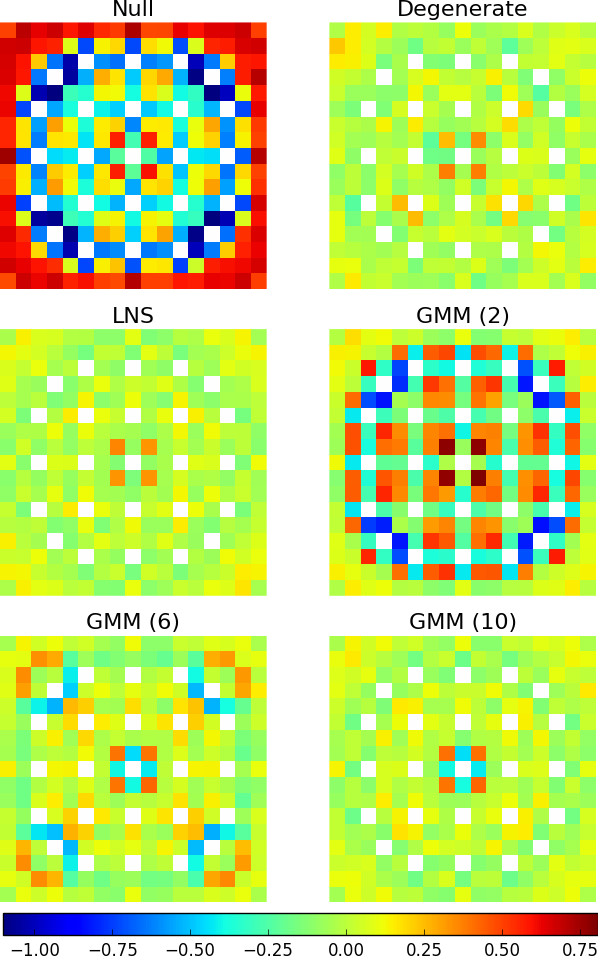
\includegraphics[width=0.9\linewidth]{figures/results/spatial/assm-16/capt-err}
\vspace{2mm}
\caption[U-238 capture errors for the 1.6\% enriched assembly]{U-238 capture percent relative errors for the 1.6\% enriched assembly with null, degenerate, \ac{LNS} and \textit{i}\ac{MGXS} spatial homogenization with 2, 6 and 10 clusters.}
\label{fig:chap11-assm-1.6-capt-err}
\end{figure}

\clearpage

\begin{figure}[h!]
\centering
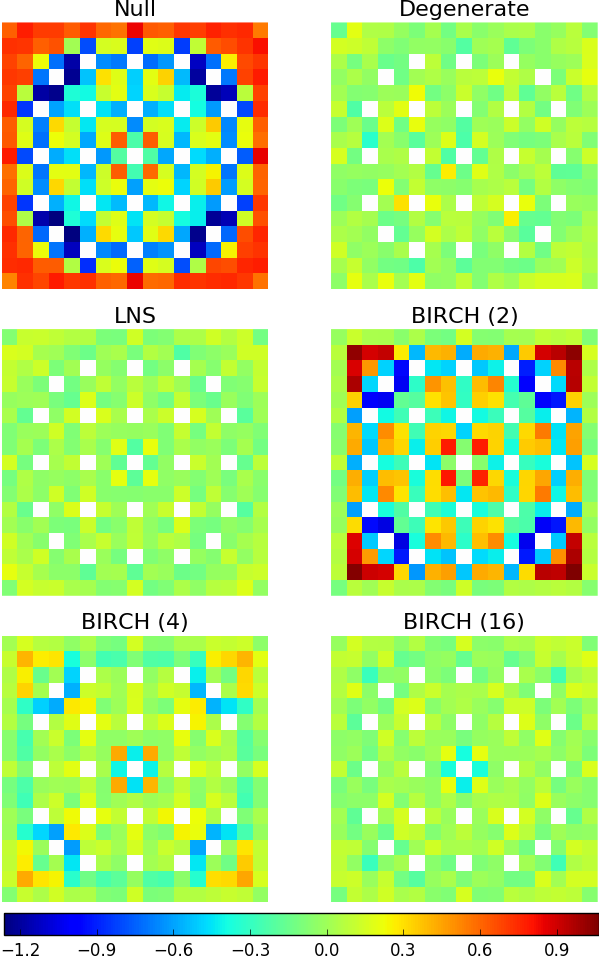
\includegraphics[width=0.9\linewidth]{figures/results/spatial/assm-31/capt-err}
\vspace{2mm}
\caption[U-238 capture errors for the 3.1\% enriched assembly]{U-238 capture percent relative errors for the 3.1\% enriched assembly with null, degenerate, \ac{LNS} and \textit{i}\ac{MGXS} spatial homogenization with 2, 6 and 10 clusters.}
\label{fig:chap11-assm-3.1-capt-err}
\end{figure}

\clearpage

\begin{figure}[h!]
\centering
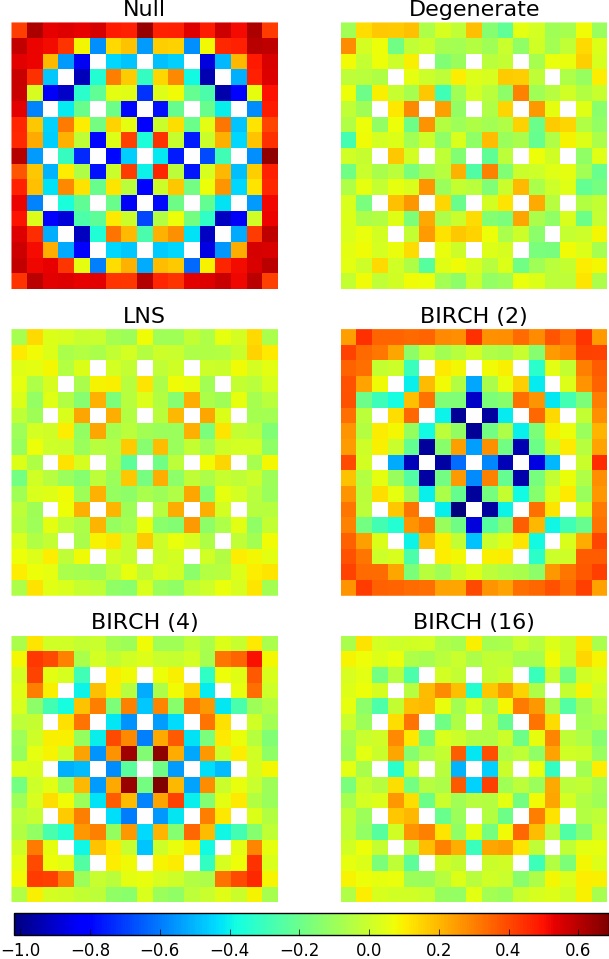
\includegraphics[width=0.9\linewidth]{figures/results/spatial/assm-31-20BPs/capt-err}
\vspace{2mm}
\caption[U-238 capture errors for the 3.1\% enriched assembly with 20 BPs]{U-238 capture percent relative errors for the 3.1\% enriched assembly with 20 \acp{BP} with null, degenerate, \ac{LNS} and \textit{i}\ac{MGXS} spatial homogenization with 2, 6 and 10 clusters.}
\label{fig:chap11-assm-3.1-20BPs-capt-err}
\end{figure}

\clearpage

\begin{figure}[h!]
\centering
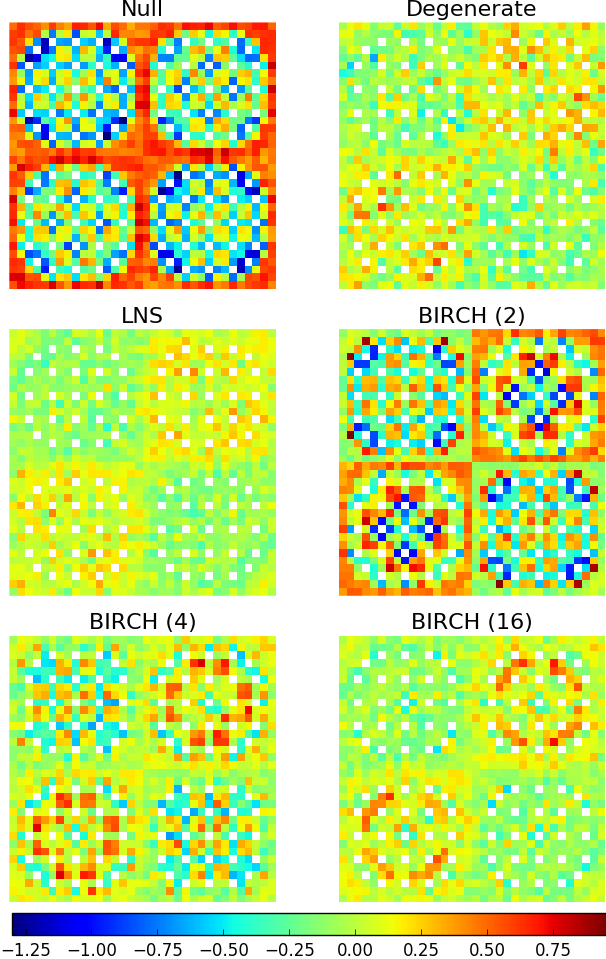
\includegraphics[width=0.9\linewidth]{figures/results/spatial/2x2/capt-err}
\vspace{2mm}
\caption[U-238 capture errors for the 2$\times$2 colorset]{U-238 capture percent relative errors for the 2$\times$2 colorset with null, degenerate, \ac{LNS} and \textit{i}\ac{MGXS} spatial homogenization with 2, 6 and 10 clusters.}
\label{fig:chap11-2x2-capt-err}
\end{figure}

\clearpage

\begin{figure}[h!]
\centering
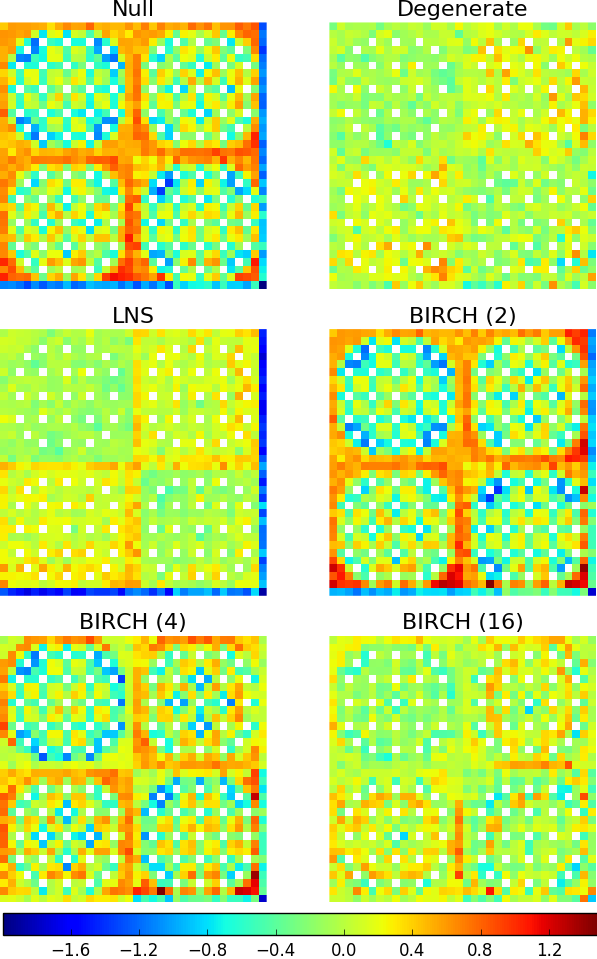
\includegraphics[width=0.9\linewidth]{figures/results/spatial/reflector/capt-err}
\vspace{2mm}
\caption[U-238 capture errors for the 2$\times$2 colorset with reflector]{U-238 capture percent relative errors for the 2$\times$2 colorset with a water reflector with null, degenerate, \ac{LNS} and \textit{i}\ac{MGXS} spatial homogenization with 2, 6 and 10 clusters.}
\label{fig:chap11-refl-capt-err}
\end{figure}

\clearpage

\begin{figure}[h!]
\centering
\begin{subfigure}{0.9\textwidth}
  \centering
  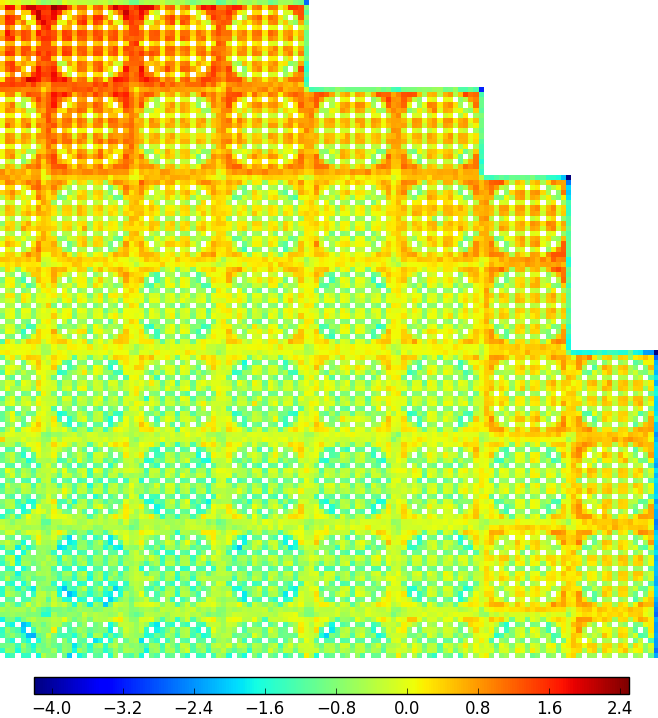
\includegraphics[width=0.65\linewidth]{figures/results/spatial/full-core/capt-err-null}
  \caption{}
  \label{fig:chap11-full-core-capt-err-null}
\end{subfigure}
\begin{subfigure}{0.9\textwidth}
  \centering
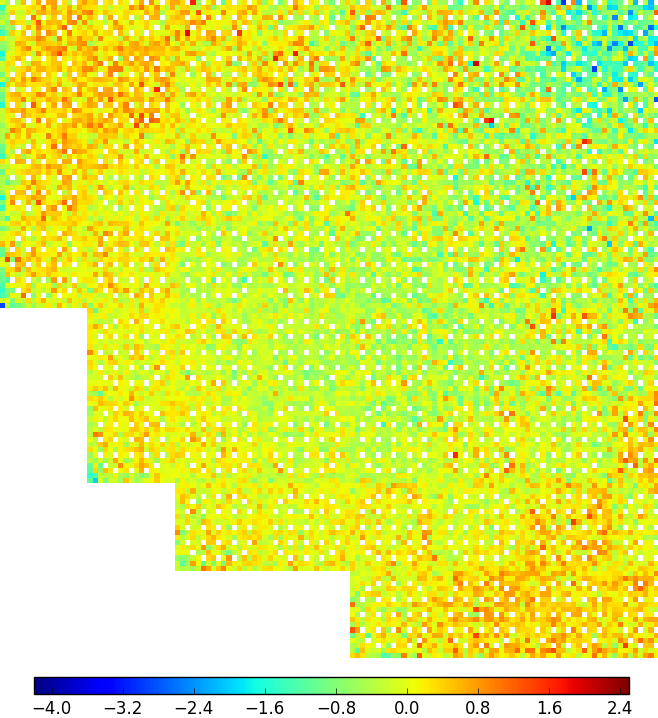
\includegraphics[width=0.65\linewidth]{figures/results/spatial/full-core/capt-err-degenerate}
  \caption{}
  \label{fig:chap11-full-core-capt-err-degenerate}
\end{subfigure}
\caption[U-238 capture rate errors for \ac{BEAVRS}]{U-238 capture percent relative errors for the quarter core \ac{BEAVRS} model with null (a) and degenerate (b) spatial homogenization.}
\label{fig:chap11-full-core-capt-err-a}
\end{figure}

\clearpage

\begin{figure}[h!]
\centering
\begin{subfigure}{0.9\textwidth}
  \centering
  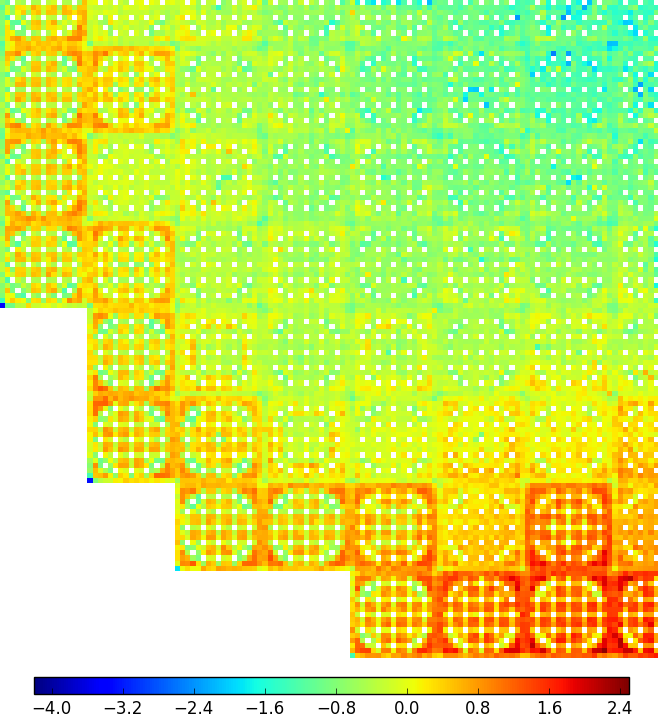
\includegraphics[width=0.65\linewidth]{figures/results/spatial/full-core/capt-err-birch-4}
  \caption{}
  \label{fig:chap11-full-core-capt-err-birch-4}
\end{subfigure}
\begin{subfigure}{0.9\textwidth}
  \centering
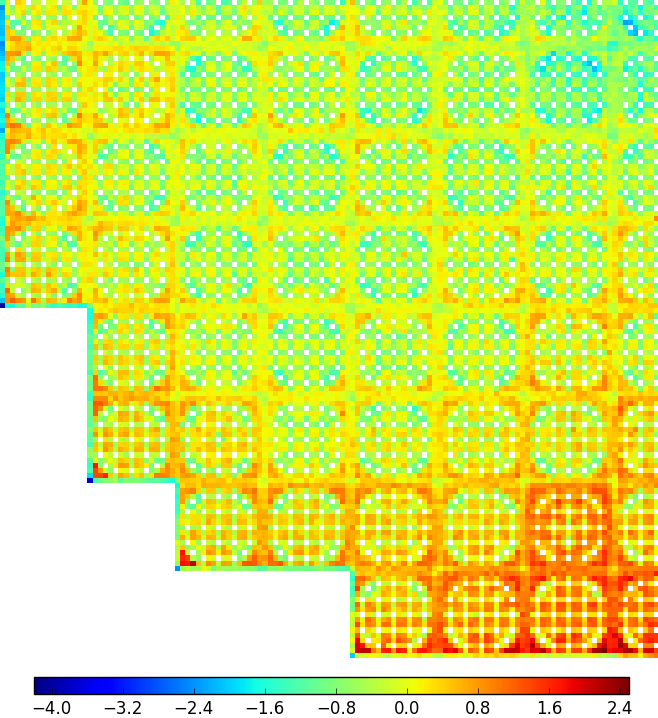
\includegraphics[width=0.65\linewidth]{figures/results/spatial/full-core/capt-err-birch-16}
  \caption{}
  \label{fig:chap11-full-core-capt-err-birch-16}
\end{subfigure}
\caption[U-238 capture rate errors for \ac{BEAVRS}]{U-238 capture percent relative errors for the quarter core \ac{BEAVRS} model with \textit{i}\ac{MGXS} spatial homogenization with BIRCH clustering of 4 (a) and 16 (b) clusters.}
\label{fig:chap11-full-core-capt-err-b}
\end{figure}

\clearpage

SUMMARY BOX

%%%%%%%%%%%%%%%%%%%%%%%%%%%%%%%%%%%%%%%%%%%
\subsubsection{Comparing OpenMOC Solutions}
\label{subsec:chap11-imgxs-capt-rates-compare}

\begin{figure}[h!]
\centering
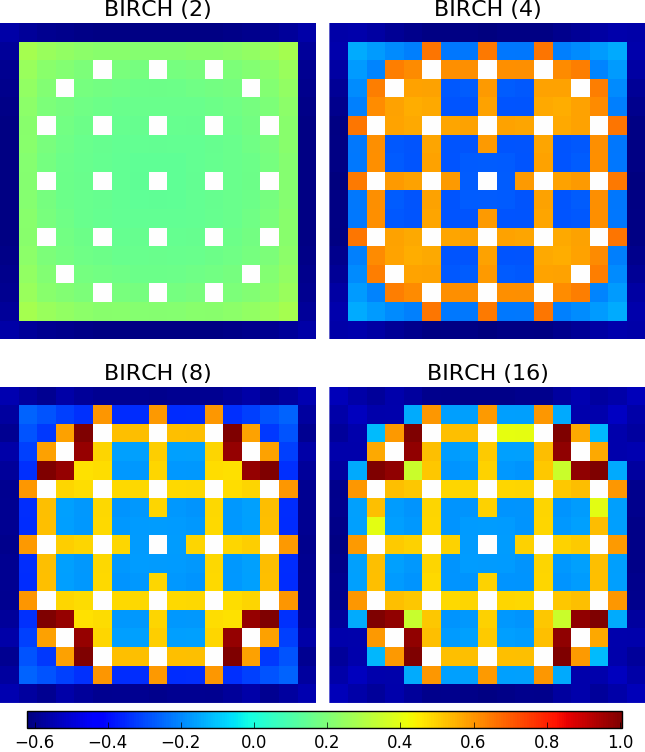
\includegraphics[width=0.9\linewidth]{figures/results/compare/assm-16/compare-capt}
\vspace{2mm}
\caption[U-238 capture rate comparison for a 1.6\% enriched assembly]{A comparison of U-238 capture rate spatial distributions for \textit{i}\ac{MGXS} and null spatial homogenization schemes for a 1.6\% enriched assembly.}
\label{fig:chap11-assm-1.6-capt-rates-comp}
\end{figure}

\clearpage

\begin{figure}[h!]
\centering
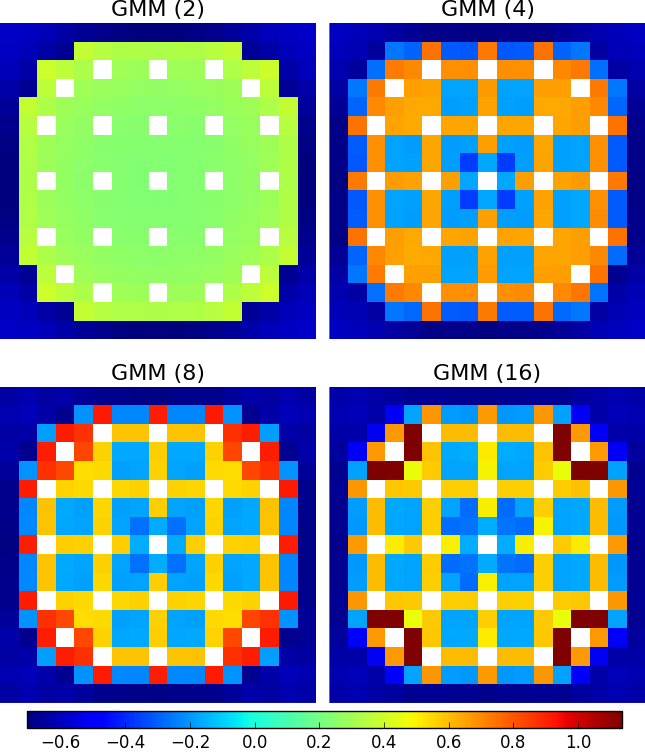
\includegraphics[width=0.9\linewidth]{figures/results/compare/assm-31/compare-capt}
\vspace{2mm}
\caption[U-238 capture rate comparison for a 3.1\% enriched assembly]{A comparison of U-238 capture rate spatial distributions for \textit{i}\ac{MGXS} and null spatial homogenization schemes for a 3.1\% enriched assembly.}
\label{fig:chap11-assm-3.1-capt-rates-comp}
\end{figure}

\clearpage

\begin{figure}[h!]
\centering
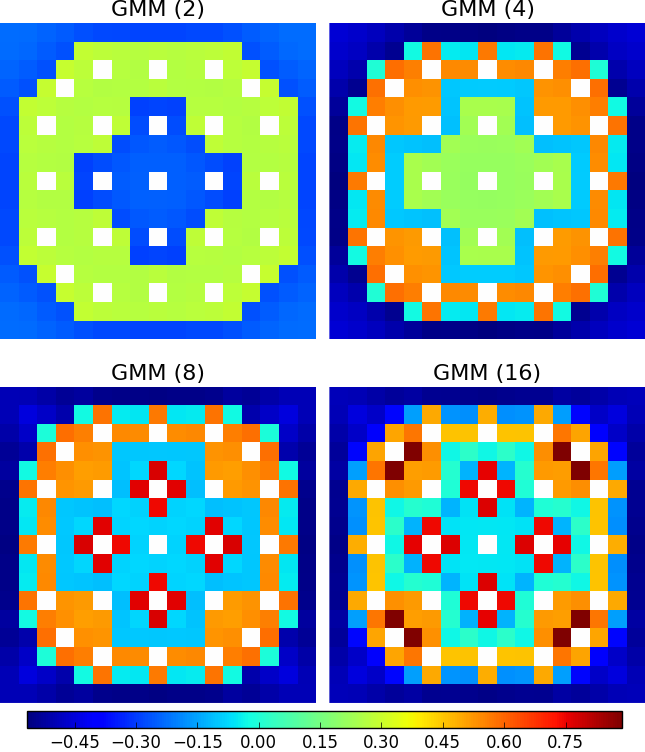
\includegraphics[width=0.9\linewidth]{figures/results/compare/assm-31-20BPs/compare-capt}
\vspace{2mm}
\caption[U-238 capture rate comparison for a 3.1\% enriched assembly with 20 BPs]{A comparison of U-238 capture rate spatial distributions for \textit{i}\ac{MGXS} and null spatial homogenization schemes for a 3.1\% enriched assembly with 20 \acp{BP}.}
\label{fig:chap11-assm-31-20BPs-capt-rates-comp}
\end{figure}
	
\clearpage

\begin{figure}[h!]
\centering
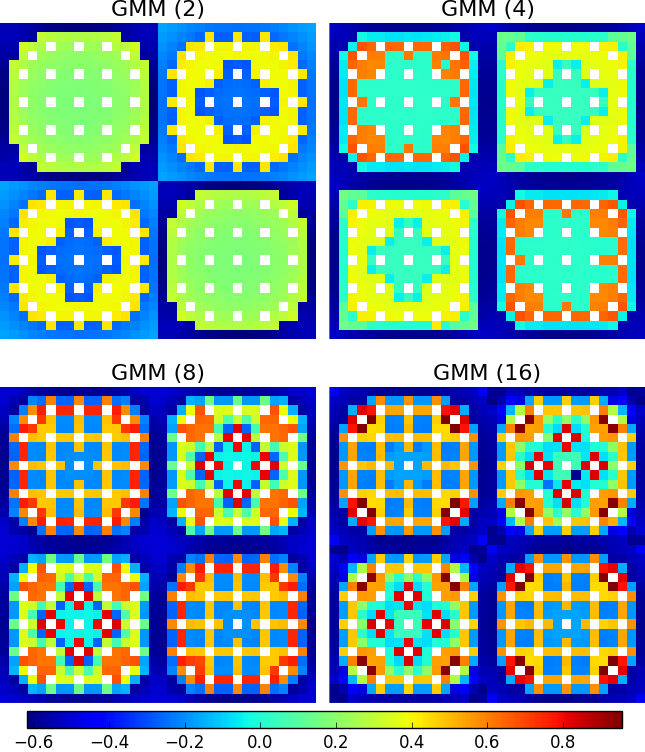
\includegraphics[width=0.9\linewidth]{figures/results/compare/2x2/compare-capt}
\vspace{2mm}
\caption[U-238 capture rate comparison for a 2$\times$2 colorset]{A comparison of U-238 capture rate spatial distributions for \textit{i}\ac{MGXS} and null spatial homogenization schemes for a 2$\times$2 colorset.}
\label{fig:chap11-assm-2x2-capt-rates-comp}
\end{figure}

\clearpage

\begin{figure}[h!]
\centering
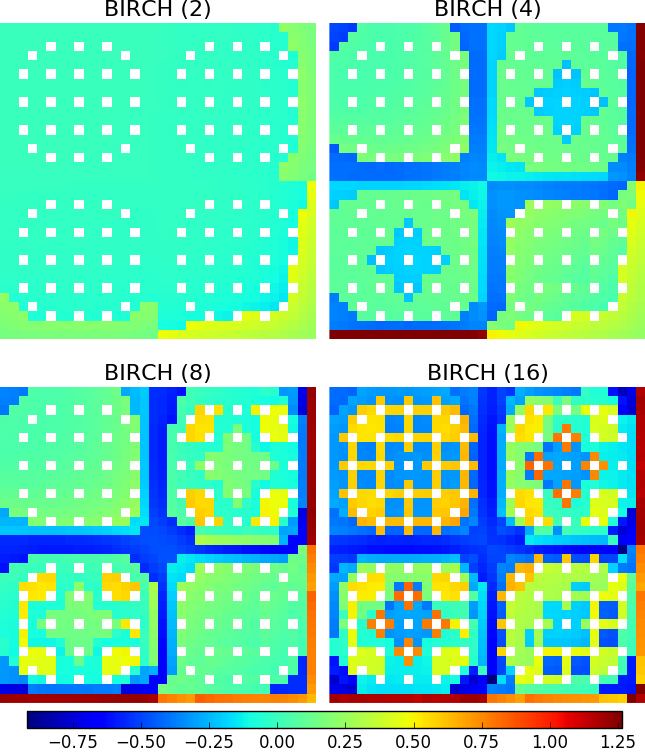
\includegraphics[width=0.9\linewidth]{figures/results/compare/reflector/compare-capt}
\vspace{2mm}
\caption[U-238 capture rate comparison for a 2$\times$2 colorset with reflector]{A comparison of U-238 capture rate spatial distributions for \textit{i}\ac{MGXS} and null spatial homogenization schemes for a 2$\times$2 colorset with a water reflector.}
\label{fig:chap11-assm-refl-capt-rates-comp}
\end{figure}

\clearpage

\begin{figure}[h!]
\centering
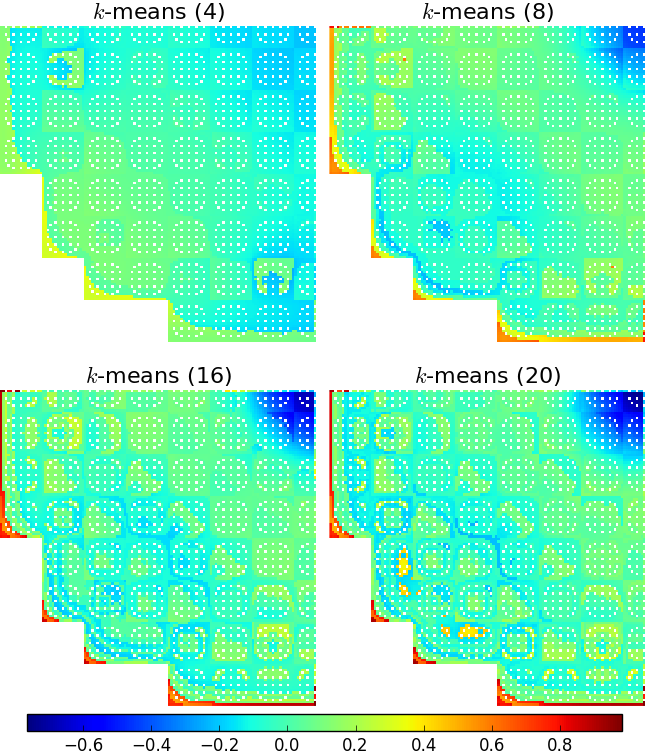
\includegraphics[width=0.9\linewidth]{figures/results/compare/full-core/compare-capt-kmeans}
\vspace{2mm}
\caption[U-238 capture rate comparison for the quarter core BEAVRS model]{A comparison of U-238 capture rate spatial distributions for \textit{i}\ac{MGXS} (\textit{with $k$-means clustering}) and null spatial homogenization schemes for the quarter core BEAVRS model.}
\label{fig:chap11-assm-full-core-capt-rates-kmeans-comp}
\end{figure}

\clearpage

\begin{figure}[h!]
\centering
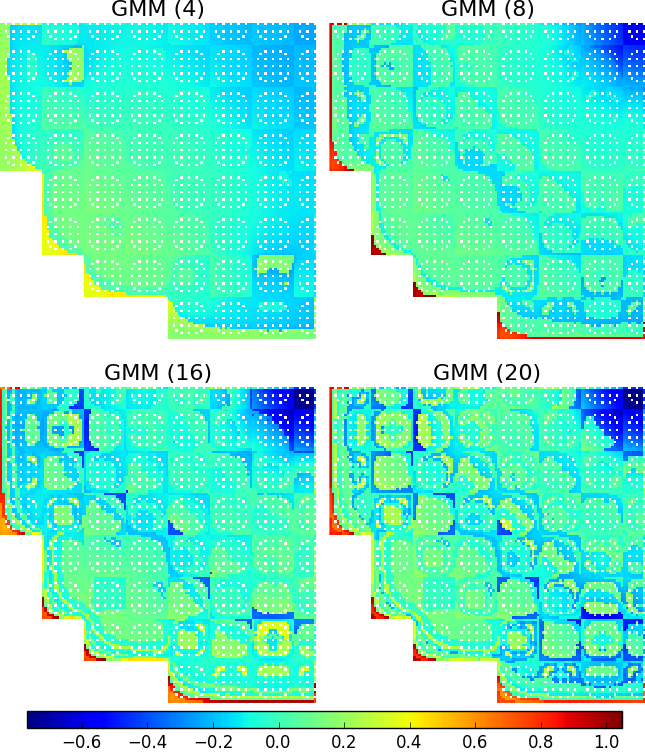
\includegraphics[width=0.9\linewidth]{figures/results/compare/full-core/compare-capt-gmm}
\vspace{2mm}
\caption[U-238 capture rate comparison for the quarter core BEAVRS model]{A comparison of U-238 capture rate spatial distributions for \textit{i}\ac{MGXS} (\textit{with \ac{GMM} clustering}) and null spatial homogenization schemes for the quarter core BEAVRS model.}
\label{fig:chap11-assm-full-core-capt-rates-gmm-comp}
\end{figure}

\clearpage

\begin{figure}[h!]
\centering
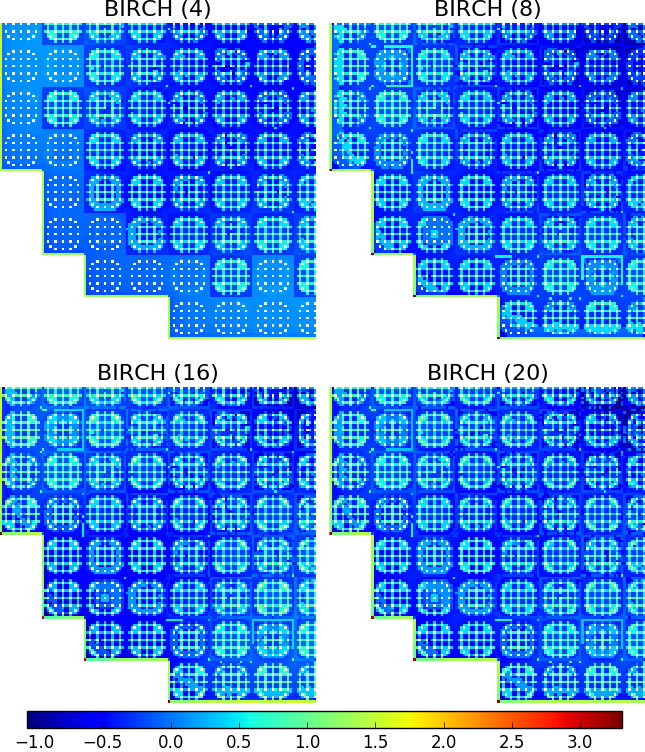
\includegraphics[width=0.9\linewidth]{figures/results/compare/full-core/compare-capt-birch}
\vspace{2mm}
\caption[U-238 capture rate comparison for the quarter core BEAVRS model]{A comparison of U-238 capture rate spatial distributions for \textit{i}\ac{MGXS} (\textit{with BIRCH clustering}) and null spatial homogenization schemes for the quarter core BEAVRS model.}
\label{fig:chap11-assm-full-core-capt-rates-birch-comp}
\end{figure}

\clearpage

SUMMARY BOX


%%%%%%%%%%%%%%%%%%%%%%%%%%%%%%%%%%%%%%%%%%%%%%%%%%%%%%%%%%%%%%%%%%%%%%%%%%%%%%%
\section{Performance with Converged MGXS}
\label{sec:chap11-improvements}

first paragraph:

-perfect batchwise: how much ``noise'' can we live with in our tally data???

OpenMC batchwise
-100,000 particles / batch - individual assemblies
-400,000 particles / batch - 2x2 and reflector??
-1,000,000 particles / batch - quarter core
-10,000 batches for assemblies and reflector
-how many for full core??
-reported statepoints for 100 logarithmically spaced batches

%%%%%%%%%%%%%%%%%%%%%%%%%%%%%%%%%%%
\subsection{Eigenvalue Convergence}
\label{subsec:chap11-eigenvalue-converge}

\clearpage

\begin{figure}[h!]
\centering
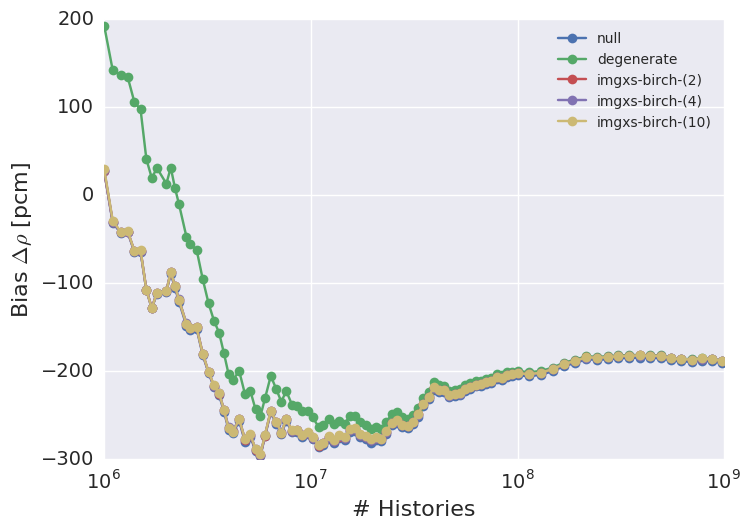
\includegraphics[width=0.87\linewidth]{figures/results/convergence/assm-16/keff-bias-evo}
\vspace{2mm}
\caption[Eigenvalue bias covergence for a 1.6\% enriched assembly]{Convergence of the eigenvalue bias $\Delta\rho$ for a 1.6\% enriched assembly.}
\label{fig:chap11-assm-1.6-eigenvalue-converge}
\end{figure}

\begin{figure}[h!]
\centering
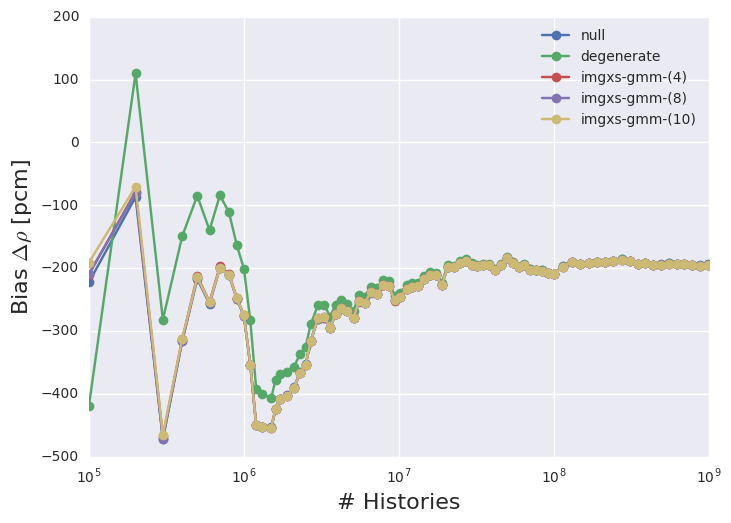
\includegraphics[width=0.87\linewidth]{figures/results/convergence/assm-31/keff-bias-evo}
\vspace{2mm}
\caption[Eigenvalue bias covergence for a 3.1\% enriched assembly]{Convergence of the eigenvalue bias $\Delta\rho$ for a 3.1\% enriched assembly.}
\label{fig:chap11-assm-3.1-eigenvalue-converge}
\end{figure}

\clearpage

\begin{figure}[h!]
\centering
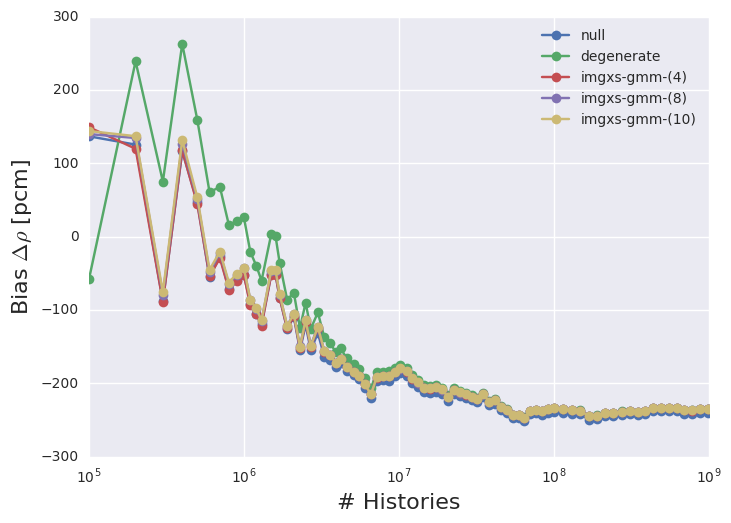
\includegraphics[width=0.87\linewidth]{figures/results/convergence/assm-31-20BPs/keff-bias-evo}
\vspace{2mm}
\caption[Eigenvalue bias covergence for a 3.1\% enriched assembly with 20 \acp{BP}]{Convergence of the eigenvalue bias $\Delta\rho$ for a 3.1\% enriched assembly with 20 \acp{BP}.}
\label{fig:chap11-assm-3.1-20BPs-eigenvalue-converge}
\end{figure}

\begin{figure}[h!]
\centering
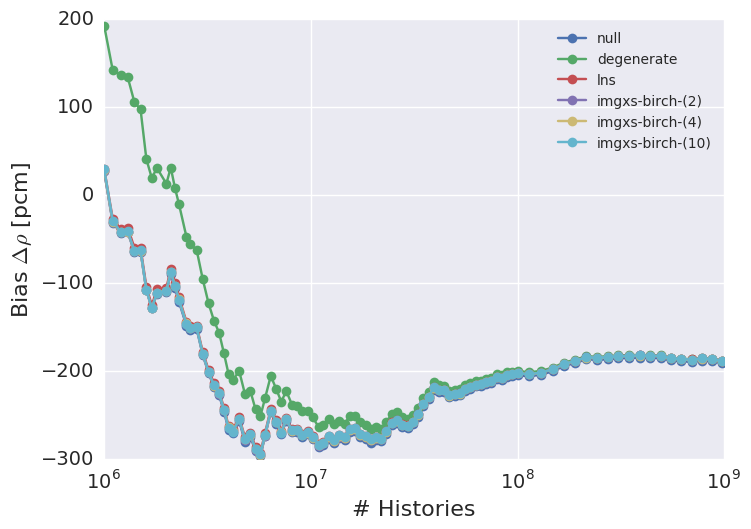
\includegraphics[width=0.87\linewidth]{figures/results/convergence/2x2/keff-bias-evo}
\vspace{2mm}
\caption[Eigenvalue bias covergence for a 2$\times$2 colorset]{Convergence of the eigenvalue bias $\Delta\rho$ for a 2$\times$2 colorset.}
\label{fig:chap11-2x2-eigenvalue-converge}
\end{figure}

\clearpage

\begin{figure}[h!]
\centering
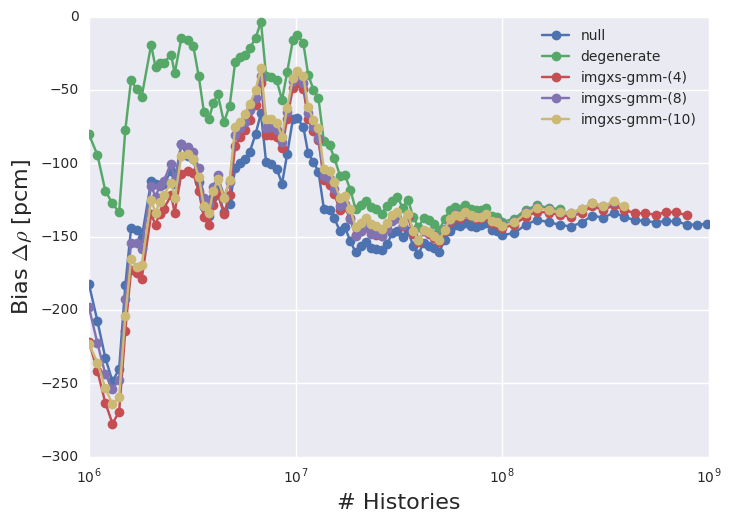
\includegraphics[width=0.87\linewidth]{figures/results/convergence/reflector/keff-bias-evo}
\vspace{2mm}
\caption[Eigenvalue bias covergence for a 2$\times$2 colorset with reflector]{Convergence of the eigenvalue bias $\Delta\rho$ for a 2$\times$2 colorset with a water reflector.}
\label{fig:chap11-refl-eigenvalue-converge}
\end{figure}

\clearpage

-plots for full core

SUMMARY BOX

%%%%%%%%%%%%%%%%%%%%%%%%%%%%%%%%%%%%%
%\subsection{Fission Rate Convergence}
%\label{subsec:chap11-fission-converge}

%%%%%%%%%%%%%%%%%%%%%%%%%%%%%%%%%%%%%%%%%%%
\subsection{U-238 Capture Rate Convergence}
\label{subsec:chap11-capture-converge}

\clearpage

\begin{figure}[h!]
\centering
\begin{subfigure}{\textwidth}
  \centering
  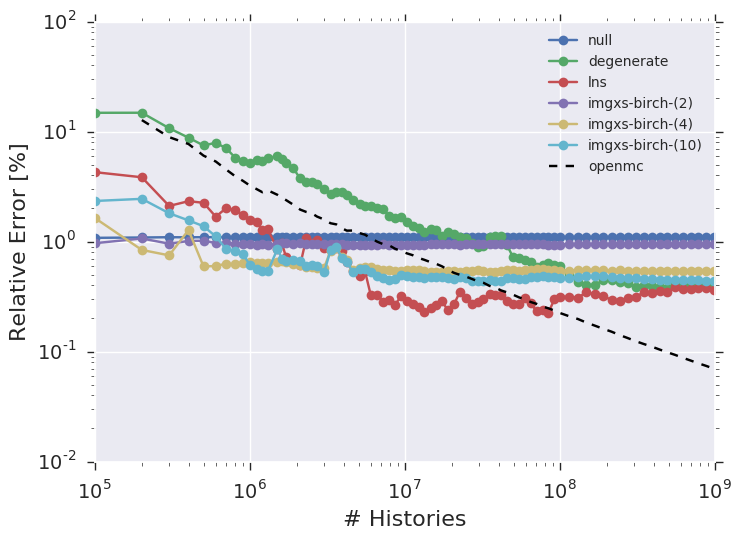
\includegraphics[width=0.9\linewidth]{figures/results/convergence/assm-16/max-capt-err-evo}
  \caption{}
  \label{fig:chap11-assm-1.6-capture-converge-max}
\end{subfigure}
\begin{subfigure}{\textwidth}
  \centering
  \includegraphics[width=0.9\linewidth]{figures/results/convergence/assm-16/mean-capt-err-evo}
  \caption{}
  \label{fig:chap11-assm-1.6-capture-converge-mean}
\end{subfigure}
\vspace{2mm}
\caption[Fission rate covergence for a 1.6\% enriched assembly]{Convergence of the max (a) and mean (b) absolute U-238 capture rate percent relative errors for a 1.6\% enriched assembly.}
\label{fig:chap11-assm-1.6-capture-converge}
\end{figure}

\clearpage

\begin{figure}[h!]
\centering
\begin{subfigure}{\textwidth}
  \centering
  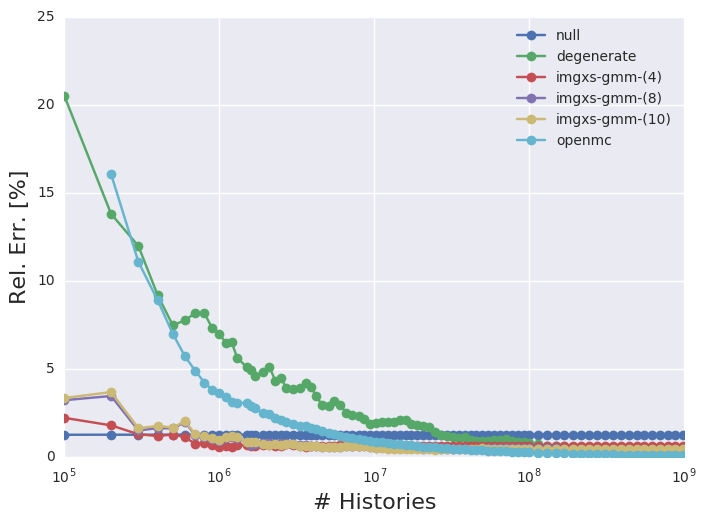
\includegraphics[width=0.9\linewidth]{figures/results/convergence/assm-31/max-capt-err-evo}
  \caption{}
  \label{fig:chap11-assm-3.1-capture-converge-max}
\end{subfigure}
\begin{subfigure}{\textwidth}
  \centering
  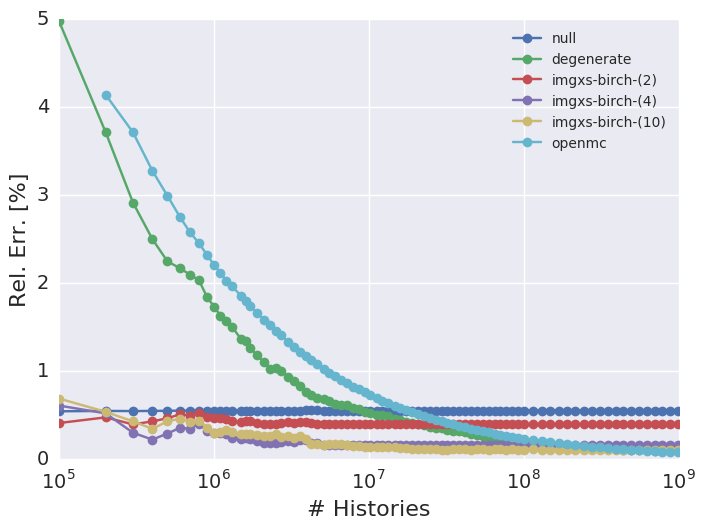
\includegraphics[width=0.9\linewidth]{figures/results/convergence/assm-31/mean-capt-err-evo}
  \caption{}
  \label{fig:chap11-assm-3.1-capture-converge-mean}
\end{subfigure}
\vspace{2mm}
\caption[Fission rate covergence for a 3.1\% enriched assembly]{Convergence of the max (a) and mean (b) absolute U-238 capture rate percent relative errors for a 3.1\% enriched assembly.}
\label{fig:chap11-assm-3.1-capture-converge}
\end{figure}

\clearpage

\begin{figure}[h!]
\centering
\begin{subfigure}{\textwidth}
  \centering
  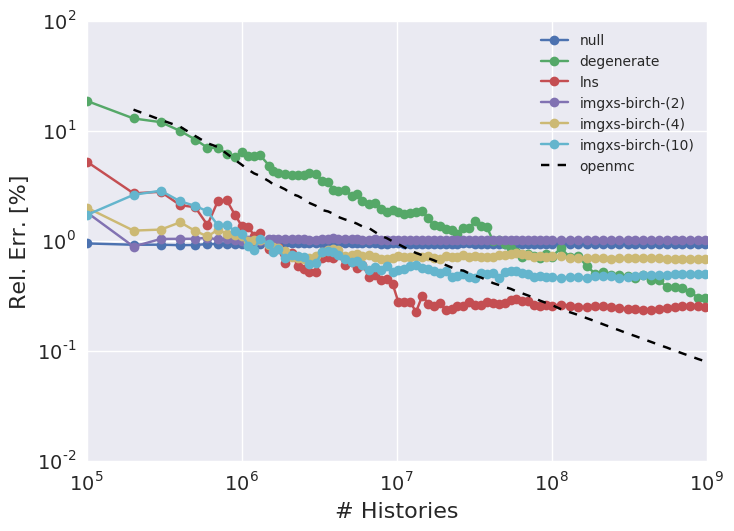
\includegraphics[width=0.9\linewidth]{figures/results/convergence/assm-31-20BPs/max-capt-err-evo}
  \caption{}
  \label{fig:chap11-assm-3.1-20BPs-capture-converge-max}
\end{subfigure}
\begin{subfigure}{\textwidth}
  \centering
  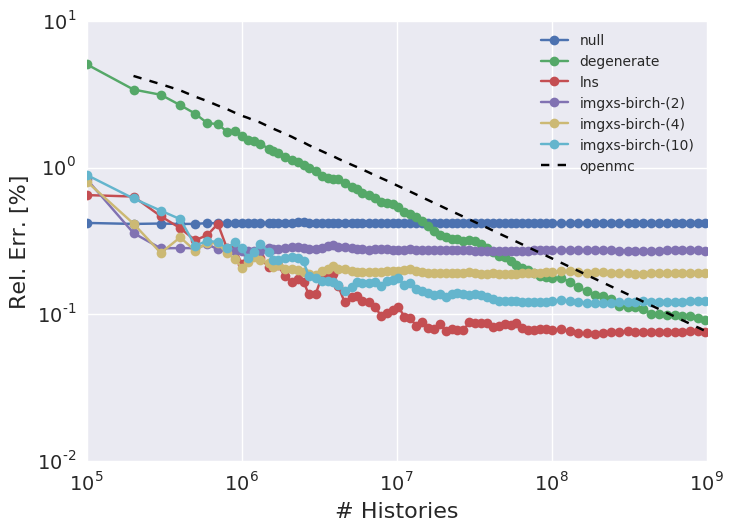
\includegraphics[width=0.9\linewidth]{figures/results/convergence/assm-31-20BPs/mean-capt-err-evo}
  \caption{}
  \label{fig:chap11-assm-3.1-20BPs-capture-converge-mean}
\end{subfigure}
\vspace{2mm}
\caption[Fission rate covergence for a 3.1\% enriched assembly with 20 \acp{BP}]{Convergence of the max (a) and mean (b) absolute U-238 capture rate percent relative errors for a 3.1\% enriched assembly with 20 \acp{BP}.}
\label{fig:chap11-assm-3.1-20BPs-capture-converge}
\end{figure}

\clearpage

\begin{figure}[h!]
\centering
\begin{subfigure}{\textwidth}
  \centering
  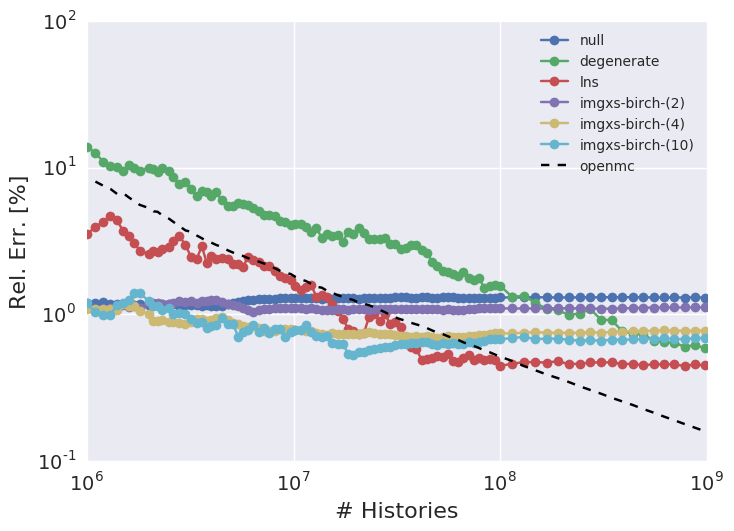
\includegraphics[width=0.9\linewidth]{figures/results/convergence/2x2/max-capt-err-evo}
  \caption{}
  \label{fig:chap11-2x2-capture-converge-max}
\end{subfigure}
\begin{subfigure}{\textwidth}
  \centering
  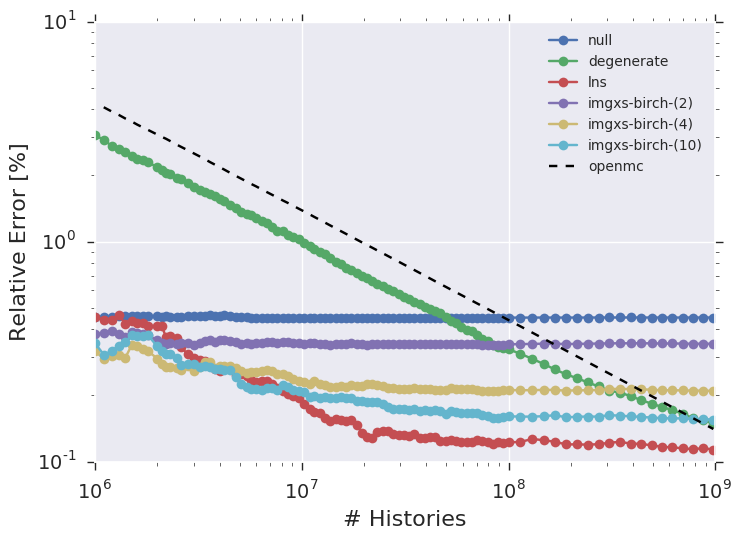
\includegraphics[width=0.9\linewidth]{figures/results/convergence/2x2/mean-capt-err-evo}
  \caption{}
  \label{fig:chap11-2x2-capture-converge-mean}
\end{subfigure}
\vspace{2mm}
\caption[Fission rate covergence for a 2$\times$2 colorset]{Convergence of the max (a) and mean (b) absolute U-238 capture rate percent relative errors for a 2$\times$2 colorset.}
\label{fig:chap11-2x2-capture-converge}
\end{figure}

\clearpage

\begin{figure}[h!]
\centering
\begin{subfigure}{\textwidth}
  \centering
  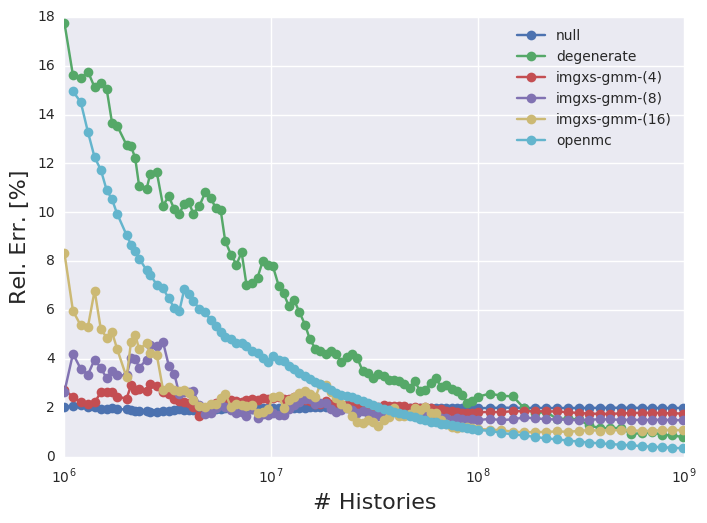
\includegraphics[width=0.9\linewidth]{figures/results/convergence/reflector/max-capt-err-evo}
  \caption{}
  \label{fig:chap11-refl-capture-converge-max}
\end{subfigure}
\begin{subfigure}{\textwidth}
  \centering
  \includegraphics[width=0.9\linewidth]{figures/results/convergence/reflector/mean-capt-err-evo}
  \caption{}
  \label{fig:chap11-refl-capture-converge-mean}
\end{subfigure}
\vspace{2mm}
\caption[Fission rate covergence for a 2$\times$2 colorset with reflector]{Convergence of the max (a) and mean (b) absolute U-238 capture rate percent relative errors for a 2$\times$2 colorset with a water reflector.}
\label{fig:chap11-refl-capture-converge}
\end{figure}

\clearpage

-full core plots

SUMMARY BOX


%%%%%%%%%%%%%%%%%%%%%%%%%%%%%%%%%%%%%%%%%%%%%%%%%%%%%%%%%%%%%%%%%%%%%%%%%%%%%%%
\section{Evaluation of Model Selection Techniques}
\label{sec:chap11-model-select}

first paragraph: objective
-

second paragraph: outline
-

%%%%%%%%%%%%%%%%%%%%%%%%%%%%%%%%%
\subsection{Davies-Bouldin Index}
\label{subsec:chap11-db-index}

\begin{figure}[h!]
\centering
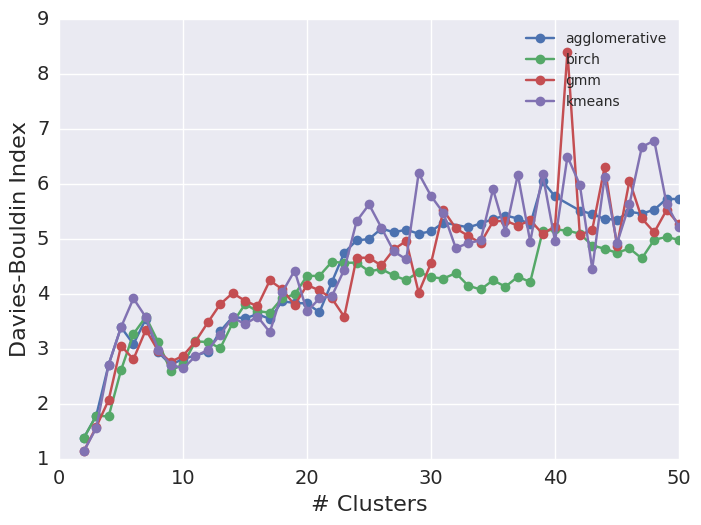
\includegraphics[width=0.87\linewidth]{figures/results/model-select/assm-16/db-combined-U238-capture-1}
\vspace{2mm}
\caption[Davies-Bouldin indices for the 1.6\% enriched assembly]{Davies-Bouldin indices for the 1.6\% enriched assembly.}
\label{fig:chap11-assm-16-db-index}
\end{figure}

\begin{figure}[h!]
\centering
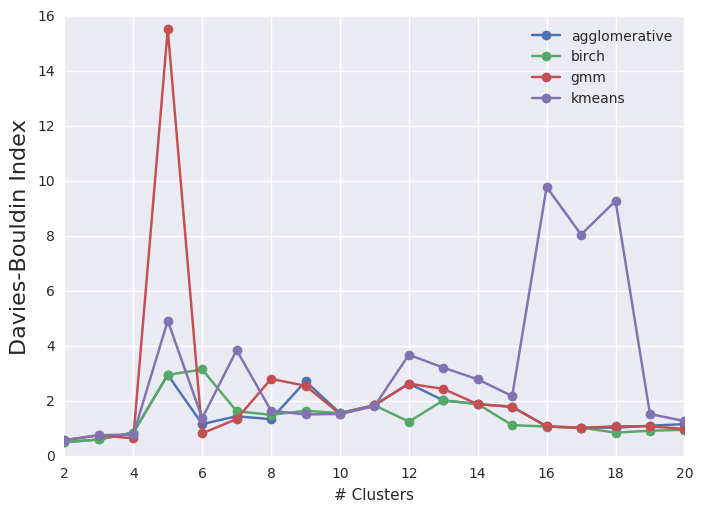
\includegraphics[width=0.87\linewidth]{figures/results/model-select/assm-31-20BPs/db-combined-U238-capture-1}
\vspace{2mm}
\caption[Davies-Bouldin indices for the 3.1\% enriched assembly with 20 BPs]{Davies-Bouldin indices for the 3.1\% enriched assembly with 20 \acp{BP}.}
\label{fig:chap11-assm-31-20BPs-db-index}
\end{figure}

\clearpage

\begin{figure}[h!]
\centering
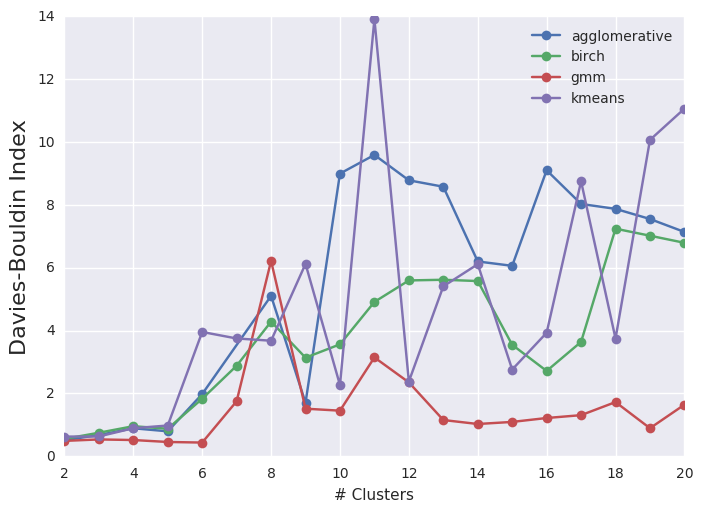
\includegraphics[width=0.87\linewidth]{figures/results/model-select/2x2/db-combined-U238-capture-1}
\vspace{2mm}
\caption[Davies-Bouldin indices for the 2$\times$2 colorset]{Davies-Bouldin indices for the 2$\times$2 colorset.}
\label{fig:chap11-2x2-db-index}
\end{figure}

\begin{figure}[h!]
\centering
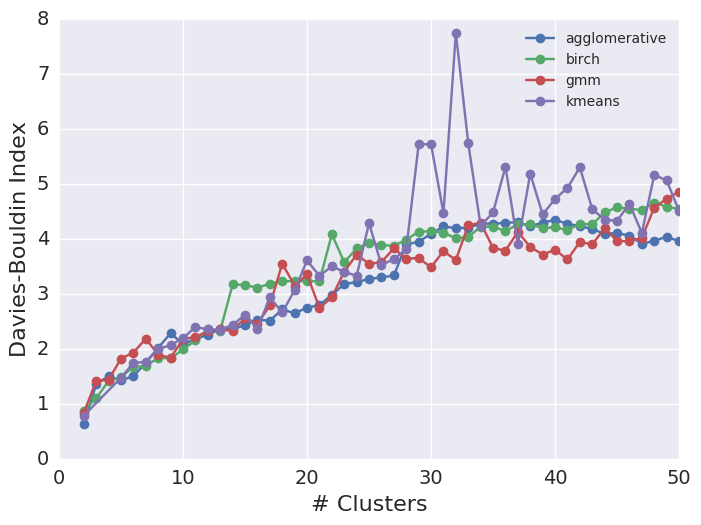
\includegraphics[width=0.87\linewidth]{figures/results/model-select/reflector/db-combined-U238-nu-fission-1}
\vspace{2mm}
\caption[Davies-Bouldin indices for the 2$\times$2 colorset with reflector]{Davies-Bouldin indices for the 2$\times$2 colorset with a water reflector.}
\label{fig:chap11-refl-db-index}
\end{figure}

\clearpage


%%%%%%%%%%%%%%%%%%%%%%%
\subsection{Dunn Index}
\label{subsec:chap11-dunn-index}

\begin{figure}[h!]
\centering
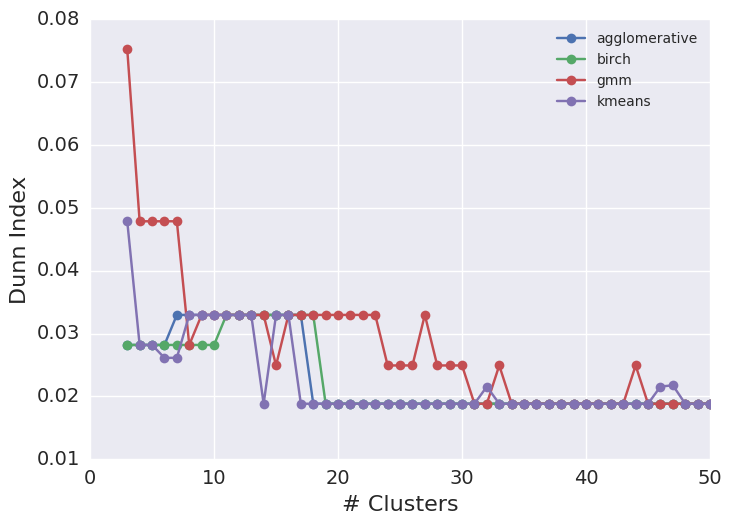
\includegraphics[width=0.87\linewidth]{figures/results/model-select/assm-16/dunn-combined-U238-capture-1}
\vspace{2mm}
\caption[Dunn indices for the 1.6\% enriched assembly]{Dunn indices for the 1.6\% enriched assembly.}
\label{fig:chap11-assm-16-dunn-index}
\end{figure}

\begin{figure}[h!]
\centering
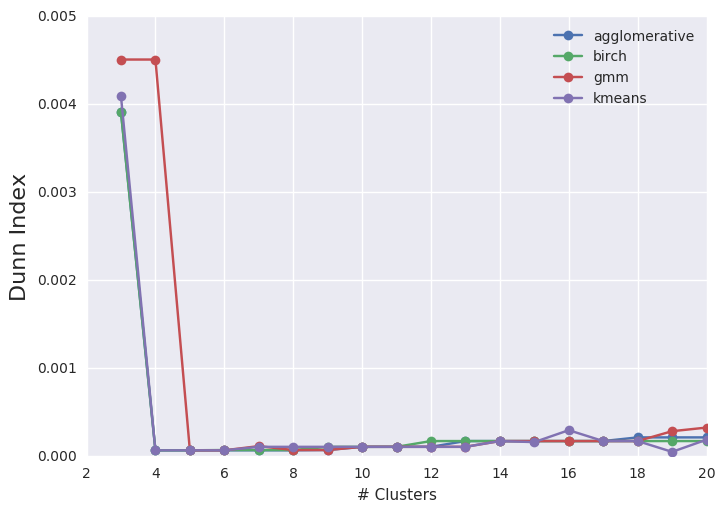
\includegraphics[width=0.87\linewidth]{figures/results/model-select/assm-31-20BPs/dunn-combined-U238-capture-1}
\vspace{2mm}
\caption[Dunn indices for the 3.1\% enriched assembly with 20 BPs]{Dunn indices for the 3.1\% enriched assembly with 20 \acp{BP}.}
\label{fig:chap11-assm-31-20BPs-dunn-index}
\end{figure}

\clearpage

\begin{figure}[h!]
\centering
\includegraphics[width=0.87\linewidth]{figures/results/model-select/2x2/dunn-combined-U238-capture-1}
\vspace{2mm}
\caption[Dunn indices for the 2$\times$2 colorset]{Dunn indices for the 2$\times$2 colorset.}
\label{fig:chap11-2x2-dunn-index}
\end{figure}

\begin{figure}[h!]
\centering
\includegraphics[width=0.87\linewidth]{figures/results/model-select/reflector/dunn-combined-U238-nu-fission-1}
\vspace{2mm}
\caption[Dunn indices for the 2$\times$2 colorset with reflector]{Dunn indices for the 2$\times$2 colorset with a water reflector.}
\label{fig:chap11-refl-dunn-index}
\end{figure}

\clearpage

%%%%%%%%%%%%%%%%%%%%%%%%%%%%%%%%%%%
\subsection{Calinski-Harabaz Index}
\label{subsec:chap11-ch-index}

\begin{figure}[h!]
\centering
\includegraphics[width=0.87\linewidth]{figures/results/model-select/assm-16/ch-combined-U238-capture-1}
\vspace{2mm}
\caption[Calinski-Harabaz indices for the 1.6\% enriched assembly]{Calinski-Harabaz indices for the 1.6\% enriched assembly.}
\label{fig:chap11-assm-16-ch-index}
\end{figure}

\begin{figure}[h!]
\centering
\includegraphics[width=0.87\linewidth]{figures/results/model-select/assm-31-20BPs/ch-combined-U238-capture-1}
\vspace{2mm}
\caption[Calinski-Harabaz indices for the 3.1\% enriched assembly with 20 BPs]{Calinski-Harabaz indices for the 3.1\% enriched assembly with 20 \acp{BP}.}
\label{fig:chap11-assm-31-20BPs-ch-index}
\end{figure}

\clearpage

\begin{figure}[h!]
\centering
\includegraphics[width=0.87\linewidth]{figures/results/model-select/2x2/ch-combined-U238-capture-1}
\vspace{2mm}
\caption[Calinski-Harabaz indices for the 2$\times$2 colorset]{Calinski-Harabaz indices for the 2$\times$2 colorset.}
\label{fig:chap11-2x2-ch-index}
\end{figure}

\begin{figure}[h!]
\centering
\includegraphics[width=0.87\linewidth]{figures/results/model-select/reflector/ch-combined-U238-nu-fission-1}
\vspace{2mm}
\caption[Calinski-Harabaz indices for the 2$\times$2 colorset with reflector]{Calinski-Harabaz indices for the 2$\times$2 colorset with a water reflector.}
\label{fig:chap11-refl-ch-index}
\end{figure}

\clearpage

%%%%%%%%%%%%%%%%%%%%%%%%%%%%%%%%%%%
\subsection{Silhouette Coefficient}
\label{subsec:chap11-silhouette-coeff}

\begin{figure}[h!]
\centering
\includegraphics[width=0.87\linewidth]{figures/results/model-select/assm-16/silhouette-combined-U238-capture-1}
\vspace{2mm}
\caption[Silhouette coefficients for the 1.6\% enriched assembly]{Silhouette coefficients for the 1.6\% enriched assembly.}
\label{fig:chap11-assm-16-silhouette-coeff}
\end{figure}

\begin{figure}[h!]
\centering
\includegraphics[width=0.87\linewidth]{figures/results/model-select/assm-31-20BPs/silhouette-combined-U238-capture-1}
\vspace{2mm}
\caption[Silhouette coefficients for the 3.1\% enriched assembly with 20 BPs]{Silhouette coefficients for the 3.1\% enriched assembly with 20 \acp{BP}.}
\label{fig:chap11-assm-31-20BPs-silhouette-coeff}
\end{figure}

\clearpage

\begin{figure}[h!]
\centering
\includegraphics[width=0.87\linewidth]{figures/results/model-select/2x2/silhouette-combined-U238-capture-1}
\vspace{2mm}
\caption[Silhouette coefficients for the 2$\times$2 colorset]{Silhouette coefficients for the 2$\times$2 colorset.}
\label{fig:chap11-2x2-silhouette-coeff}
\end{figure}

\begin{figure}[h!]
\centering
\includegraphics[width=0.87\linewidth]{figures/results/model-select/reflector/silhouette-combined-U238-nu-fission-1}
\vspace{2mm}
\caption[Silhouette coefficients for the 2$\times$2 colorset with reflector]{Silhouette coefficients for the 2$\times$2 colorset with a water reflector.}
\label{fig:chap11-refl-silhouette-coeff}
\end{figure}

\clearpage

%%%%%%%%%%%%%%%%%%%%%%%%%%%%%%%%%%%%%%%%%%%
\subsection{Bayesian Information Criterion}
\label{subsec:chap11-bic}

\begin{figure}[h!]
\centering
\includegraphics[width=0.87\linewidth]{figures/results/model-select/assm-16/bic-combined-U238-capture-1}
\vspace{2mm}
\caption[Silhouette coefficients for the 1.6\% enriched assembly]{Bayesian Information Criteria (BIC) for the 1.6\% enriched assembly.}
\label{fig:chap11-assm-16-bic}
\end{figure}

\begin{figure}[h!]
\centering
\includegraphics[width=0.87\linewidth]{figures/results/model-select/assm-31-20BPs/bic-combined-U238-capture-1}
\vspace{2mm}
\caption[Silhouette coefficients for the 3.1\% enriched assembly with 20 BPs]{Bayesian Information Criteria (BIC) for the 3.1\% enriched assembly with 20 \acp{BP}.}
\label{fig:chap11-assm-31-20BPs-bic}
\end{figure}

\clearpage

\begin{figure}[h!]
\centering
\includegraphics[width=0.87\linewidth]{figures/results/model-select/2x2/bic-combined-U238-capture-1}
\vspace{2mm}
\caption[BIC for the 2$\times$2 colorset]{Bayesian Information Criteria (BIC) for the 2$\times$2 colorset.}
\label{fig:chap11-2x2-bic}
\end{figure}

\begin{figure}[h!]
\centering
\includegraphics[width=0.87\linewidth]{figures/results/model-select/reflector/bic-combined-U238-nu-fission-1}
\vspace{2mm}
\caption[BIC for the 2$\times$2 colorset with reflector]{Bayesian Information Criteria (BIC) for the 2$\times$2 colorset with a water reflector.}
\label{fig:chap11-refl-bic}
\end{figure}

\clearpage

SUMMARY BOX!!!

%%%%%%%%%%%%%%%%%%%%%%%%%%%%%%%%%%%%%%%%%%%%%%%%%%%%%%%%%%%%%%%%%%%%%%%%%%%%%%%
\section{Synthesis}
\label{sec:chap11-synthesis}

-bring it all together - what does it all mean??
-recall Fig. 10-1
  -quantify how much faster \textit{i}\ac{MGXS} would be then full core MC
  -table of runtimes

-plot of model complexity with generalization error by batch

-OpenMOC runtimes for litmus-only feature selection with GMMs with 10 clusters

OpenMC particles / sec / core
benchmark         no MGXs        MGXS
1.6               2673.3         1154.4
3.1               3012.9         1265.1
3.1 BPs           3051.4         1011.4
2x2               2976.3          784.9
reflector         3004.6          795.6
quarter core      2361.5          622.2

-use particle tracking rate to compute total time
  -read number of batches from the convergence plots as the max(max err,mean err) <= degenerate err
  -multiply number of batches by particle tracking rate
  -this uses the tracking rate without MGXS for the ``reference''
  -this use the tracking rate with MGXS for all others
  -10 clusters each???

\begin{table}[ht!]
  \centering
  \caption[OpenMOC eigenvalue bias for litmus-only feature selection]{OpenMOC eigenvalue bias $\Delta\rho$ for \textit{i}\ac{MGXS} spatial homogenization with litmus-only feature selection.}
  \small
  \label{table:chap11-runtimes}
  \vspace{6pt}
  \begin{tabular}{l l R{2.5cm} S[table-format=3.2] S[table-format=3.2] S[table-format=3.2]}
  \toprule
  \rowcolor{lightgray}
  & & & \multicolumn{3}{c}{\cellcolor{lightgray} \bf Runtime [core-hours]} \\
  \multirow{-2}{*}{\cellcolor{lightgray} \bf Benchmark} &
  \multirow{-2}{*}{\cellcolor{lightgray} \bf Scheme} &
  \multirow{-2}{*}{\cellcolor{lightgray} \bf \# Particles} &
  \multicolumn{1}{c}{\cellcolor{lightgray} \bf OpenMC} &
  \multicolumn{1}{c}{\cellcolor{lightgray} \bf OpenMOC} &
  \multicolumn{1}{c}{\cellcolor{lightgray} \bf Total} \\
  \midrule
\multirow{4}{*}{\parbox{2.5cm}{1.6\% Assm}} & Reference & 550,000,000 & 57.2 & & 57.2 \\
& Null & 100,000 & 0.02 & 0.36 & 0.38 \\
& Degenerate & 115,000,000 & 27.7 & 0.40 & 28.1 \\
& \textit{i}\ac{MGXS} & 4,000,000 & 0.96 & 0.38 & 1.34 \\
  \midrule
\multirow{4}{*}{\parbox{2.5cm}{3.1\% Assm}} & Reference & 550,000,000 & 50.7 & & 50.7 \\
& Null & 100,000 & 0.02 & 0.40 & 0.42 \\
& Degenerate & 115,000,000 & 25.3 & 0.40 & 25.7 \\
& \textit{i}\ac{MGXS} & 4,000,000 & 0.88 & 0.37 & 1.25 \\
  \midrule
\multirow{4}{*}{\parbox{2.5cm}{3.1\% Assm w/ 20 \acp{BP}}} & Reference & 550,000,000 & 50.1 & & 50.1 \\
& Null & 100,000 & 0.02 & 0.41 & 0.43 \\
& Degenerate & 115,000,000 & 27.7 & 0.41 & 28.1 \\
& \textit{i}\ac{MGXS} & 4,000,000 & 0.96 & 0.42 & 1.38 \\
  \midrule
\multirow{4}{*}{\parbox{2.5cm}{2$\times$2 Colorset}} & Reference & 8,755,000 & 81.7 & & 81.7 \\
& Null & 100,000 & 0.04 & 2.00 & 2.03 \\
& Degenerate & 700,000,000 & 248 & 2.29 & 250 \\
& \textit{i}\ac{MGXS} & 10,000,000 & 3.54 & 1.96 & 5.50 \\
  \midrule
\multirow{4}{*}{\parbox{2.5cm}{2$\times$2 Colorset w/ Reflector}} & Reference & & & & \\
& Null & & & 5.07 & \\
& Degenerate & & & 5.36 & \\
& \textit{i}\ac{MGXS} & & & 4.90 & \\
  \midrule
\multirow{4}{*}{\parbox{2.5cm}{BEAVRS Quarter Core}} & Reference & & & & \\
& Null & & & 419 & \\
& Degenerate & & & 426 & \\
& \textit{i}\ac{MGXS} & & & 423 & \\
  \bottomrule
\end{tabular}
\end{table}

SUMMARY BOX!!!